% main.tex
% Main LaTeX document for Mobile Anyons from Fusion Categories
% This file includes all section files modularly

\documentclass[11pt,a4paper]{article}

% ============================================================
% Packages
% ============================================================
\usepackage[utf8]{inputenc}
\usepackage[T1]{fontenc}
\usepackage{amsmath,amssymb,amsthm}
\usepackage{mathtools}
\usepackage{physics}  % for bra-ket notation
\usepackage{enumitem}
\usepackage{booktabs}
\usepackage[dvipsnames]{xcolor}  % for colors (load before hyperref)
\usepackage{hyperref}
\usepackage{cleveref}
\usepackage[margin=1in]{geometry}
\usepackage{listings}  % for code listings

% ============================================================
% TikZ Style Library for Fusion Category Diagrams
% ============================================================
% tikz_styles.tex
% TikZ Style Library for Mobile Anyons from Fusion Categories
% ============================================================
% This file provides a comprehensive collection of TikZ styles and macros
% for drawing fusion category diagrams, including:
%   - Fusion trees and morphism diagrams
%   - F-moves (associators) and pentagon equations
%   - R-moves (braiding) and hexagon equations
%   - Evaluation/coevaluation (cups and caps)
%   - Anyon chains and string diagrams

% ============================================================
% Required TikZ Libraries
% ============================================================
\usepackage{tikz}
\usetikzlibrary{
    positioning,           % Relative positioning
    shapes.geometric,      % Geometric shapes
    decorations.markings,  % Arrow decorations on paths
    decorations.pathmorphing, % Wavy/snake lines
    decorations.pathreplacing, % Braces
    arrows,                % Arrow tips
    arrows.meta,           % Modern arrow tips
    knots,                 % Knot crossings for braiding
    calc,                  % Coordinate calculations
    shapes,                % Additional shapes
    backgrounds,           % Background layers
    fit                    % Fitting nodes
}

% ============================================================
% Color Definitions
% ============================================================
% Primary colors for objects/anyons
\definecolor{AnyonRed}{RGB}{221, 6, 0}
\definecolor{AnyonBlue}{RGB}{15, 105, 197}
\definecolor{AnyonGreen}{RGB}{11, 170, 21}
\definecolor{AnyonOrange}{RGB}{238, 143, 0}

% Gray for boxes and backgrounds
\definecolor{LightGray}{RGB}{220,220,220}
\definecolor{MediumGray}{RGB}{180,180,180}

% ============================================================
% Basic Arrow Styles for String Diagrams
% ============================================================
% Arrow at 60% along the path (standard direction)
\tikzset{->-/.style={
    decoration={markings, mark=at position .6 with {\arrow[>=stealth]{>}}},
    postaction={decorate}
}}

% Arrow at 52% (for certain diagram types)
\tikzset{-->--/.style={
    decoration={markings, mark=at position .52 with {\arrow[>=stealth]{>}}},
    postaction={decorate}
}}

% Reverse arrow at 60%
\tikzset{-<-/.style={
    decoration={markings, mark=at position .6 with {\arrow[>=stealth]{<}}},
    postaction={decorate}
}}

% Arrow at 50% (centered)
\tikzset{->>-/.style={
    decoration={markings, mark=at position .5 with {\arrow[>=stealth]{>}}},
    postaction={decorate}
}}

\tikzset{-<<-/.style={
    decoration={markings, mark=at position .5 with {\arrow[>=stealth]{<}}},
    postaction={decorate}
}}

% Arrow at different positions for longer strands
\tikzset{->>>-/.style={
    decoration={markings, mark=at position .5 with {\arrow[>=stealth]{>}}},
    postaction={decorate}
}}

\tikzset{-<<<-/.style={
    decoration={markings, mark=at position .4 with {\arrow[>=stealth]{<}}},
    postaction={decorate}
}}

% ============================================================
% Morphism Box Styles
% ============================================================
% Standard morphism box (gray rounded rectangle)
\tikzset{morphism box/.style={
    rectangle,
    draw,
    rounded corners,
    fill=LightGray,
    text centered,
    minimum height=0.7cm,
    minimum width=0.9cm,
    font=\small
}}

% Small morphism box
\tikzset{morphism box small/.style={
    morphism box,
    minimum height=0.5cm,
    minimum width=0.6cm,
    font=\scriptsize
}}

% Large morphism box (for composite morphisms)
\tikzset{morphism box large/.style={
    morphism box,
    minimum height=1cm,
    minimum width=1.2cm
}}

% ============================================================
% Fusion Vertex Styles
% ============================================================
% Filled vertex (standard trivalent vertex)
\tikzset{fusion vertex/.style={
    circle,
    fill=black,
    inner sep=1.5pt,
    outer sep=0pt
}}

% Empty vertex (for unfilled vertices)
\tikzset{fusion vertex empty/.style={
    circle,
    draw,
    fill=white,
    inner sep=1.5pt,
    outer sep=0pt
}}

% ============================================================
% Label Styles
% ============================================================
% Object labels (on strands)
\tikzset{object label/.style={
    font=\small,
    fill=white,
    inner sep=1pt
}}

% Vertex labels (multiplicity indices at vertices)
\tikzset{vertex label/.style={
    font=\tiny,
    fill=white,
    inner sep=0.5pt
}}

% Coefficient labels (for F-matrices, R-matrices)
\tikzset{coeff label/.style={
    font=\footnotesize,
    midway,
    fill=white,
    inner sep=1pt
}}

% ============================================================
% Commutative Diagram Arrow Style
% ============================================================
\tikzset{cd arrow/.style={
    ->,
    >=stealth,
    thick
}}

% Pentagon/Hexagon diagram arrow
\tikzset{
    pentagon arrow/.style={
        postaction={decorate},
        decoration={markings, mark=at position 1 with {\arrow[scale=1,thick]{>}}}
    }
}

% ============================================================
% MACROS FOR COMMON DIAGRAMS
% ============================================================

% ------------------------------------------------------------
% Trivalent Vertex (splitting): c -> a tensor b
% Usage: \trivalentvertex{a}{b}{c}
% ------------------------------------------------------------
\newcommand{\trivalentvertex}[3]{%
\begin{tikzpicture}[scale=0.7,baseline={(0,0.2)}]
    \draw (0,0) -- +(90:1) node[above] {\small $#3$};
    \draw (0,0) -- +(225:1) node[below] {\small $#1$};
    \draw (0,0) -- +(315:1) node[below] {\small $#2$};
\end{tikzpicture}%
}

% ------------------------------------------------------------
% Left-associative Fusion Tree: ((a,b)_e, c)_d
% Usage: \fuselefttree{a}{b}{e}{c}{d}
% ------------------------------------------------------------
\newcommand{\fuselefttree}[5]{%
\begin{tikzpicture}[scale=0.425,baseline={(0,0.4)}]
    \draw (0,0) node[below] {\small $#1$} -- (1.5,1.5) -- (3,0) node[below] {\small $#4$};
    \draw (0.75,0.75) -- (1.5,0) node[below] {\small $#2$};
    \draw (0.7,1.6) node {\small $#3$};
    \draw (1.5,1.5) -- (1.5,2.25) node[above] {\small $#5$};
\end{tikzpicture}%
}

% ------------------------------------------------------------
% Right-associative Fusion Tree: (a, (b,c)_e)_d
% Usage: \fuserighttree{a}{b}{e}{c}{d}
% ------------------------------------------------------------
\newcommand{\fuserighttree}[5]{%
\begin{tikzpicture}[scale=0.425,baseline={(0,0.4)}]
    \draw (0,0) node[below] {\small $#1$} -- (1.5,1.5) -- (3,0) node[below] {\small $#4$};
    \draw (2.25,0.75) -- (1.5,0) node[below] {\small $#2$};
    \draw (2.3,1.6) node {\small $#3$};
    \draw (1.5,1.5) -- (1.5,2.25) node[above] {\small $#5$};
\end{tikzpicture}%
}

% ------------------------------------------------------------
% F-move (Associator) Equation
% Displays: left tree = sum_f F * right tree
% Usage: \Fmoveequation{a}{b}{c}{d}{e}{f}
% ------------------------------------------------------------
\newcommand{\Fmoveequation}[6]{%
\begin{tikzpicture}[baseline=(current bounding box.center),scale=0.9]
    % Left tree: ((a b)_e c)_d
    \begin{scope}
        \draw (0,0.5) -- (0,1);
        \draw (0,1) -- (-0.5,1.5);
        \draw (-0.5,1.5) -- (-1,2);
        \draw (-0.5,1.5) -- (0,2);
        \draw (0,1) -- (0.5,1.5);
        \draw (0.5,1.5) -- (1,2);
        \node at (0,0.25) {\small $#4$};
        \node at (-1,2.25) {\small $#1$};
        \node at (0,2.25) {\small $#2$};
        \node at (1,2.25) {\small $#3$};
        \node at (-0.5,1.1) {\small $#5$};
    \end{scope}
    % Equals sign
    \node at (1.8,1.25) {$=\displaystyle\sum_{#6} \left(F_{#4}^{#1#2#3}\right)_{#6#5}$};
    % Right tree: (a (b c)_f)_d
    \begin{scope}[xshift=5.5cm]
        \draw (0,0.5) -- (0,1);
        \draw (0,1) -- (-0.5,1.5);
        \draw (-0.5,1.5) -- (-1,2);
        \draw (0.5,1.5) -- (0,2);
        \draw (0,1) -- (0.5,1.5);
        \draw (0.5,1.5) -- (1,2);
        \node at (0,0.25) {\small $#4$};
        \node at (-1,2.25) {\small $#1$};
        \node at (0,2.25) {\small $#2$};
        \node at (1,2.25) {\small $#3$};
        \node at (0.5,1.1) {\small $#6$};
    \end{scope}
\end{tikzpicture}%
}

% ------------------------------------------------------------
% Evaluation (Cup): X* tensor X -> 1
% Usage: \evalcup{X}
% ------------------------------------------------------------
\newcommand{\evalcup}[1]{%
\begin{tikzpicture}[scale=0.85,baseline=(current bounding box.center)]
    \node at (-0.3,0) {$#1^*$};
    \node at (1.7,0) {$#1$};
    \draw (0,0) arc (180:0:0.7);
\end{tikzpicture}%
}

% ------------------------------------------------------------
% Coevaluation (Cap): 1 -> X tensor X*
% Usage: \coevalcap{X}
% ------------------------------------------------------------
\newcommand{\coevalcap}[1]{%
\begin{tikzpicture}[scale=0.85,baseline=(current bounding box.center)]
    \node at (-0.3,0) {$#1$};
    \node at (1.7,0) {$#1^*$};
    \draw (0,0) arc (-180:0:0.7);
\end{tikzpicture}%
}

% ------------------------------------------------------------
% Left Zigzag Identity (Snake equation)
% Usage: \leftzigzag{X}
% ------------------------------------------------------------
\newcommand{\leftzigzag}[1]{%
\begin{tikzpicture}[baseline=(current bounding box.center)]
    \draw (0,0) -- (0,1);
    \draw (0,1) arc (0:180:0.4);
    \draw (-0.8,1) arc (0:-180:0.4);
    \draw (-1.6,1) -- (-1.6,2);
    \node at (0.25,0) {$#1$};
    \node at (-1.85,2) {$#1$};
    \node at (-1.05,1) {$#1^*$};
\end{tikzpicture}%
}

% ------------------------------------------------------------
% Right Zigzag Identity (Snake equation)
% Usage: \rightzigzag{X}
% ------------------------------------------------------------
\newcommand{\rightzigzag}[1]{%
\begin{tikzpicture}[baseline=(current bounding box.center)]
    \draw (0,0) -- (0,1);
    \draw (0,1) arc (180:0:0.4);
    \draw (0.8,1) arc (-180:0:0.4);
    \draw (1.6,1) -- (1.6,2);
    \node at (-0.25,0) {$#1^*$};
    \node at (1.85,2) {$#1^*$};
    \node at (1.05,1) {$#1$};
\end{tikzpicture}%
}

% ------------------------------------------------------------
% Simple Braiding (Over-crossing): X crosses over Y
% Usage: \braidingover{X}{Y}
% ------------------------------------------------------------
\newcommand{\braidingover}[2]{%
\begin{tikzpicture}[scale=0.85,baseline=(current bounding box.center)]
    \node at (-0.75,0.35) {$#1$};
    \node at (-0.75,2.65) {$#2$};
    \node at (0.75,0.35) {$#2$};
    \node at (0.75,2.65) {$#1$};
    \draw (-0.4,0.2) -- (-0.4,0.5);
    \draw (-0.4,2.5) -- (-0.4,2.8);
    \draw (0.4,0.2) -- (0.4,0.5);
    \draw (0.4,2.5) -- (0.4,2.8);
    \begin{knot}[flip crossing/.list={8},consider self intersections=true,ignore endpoint intersections=false]
        \strand (-0.4,0.5)to[out=90,in=270](0.4,2.5);
        \strand (0.4,0.5)to[out=90,in=270](-0.4,2.5);
    \end{knot}
\end{tikzpicture}%
}

% ------------------------------------------------------------
% Inverse Braiding (Under-crossing): X crosses under Y
% Usage: \braidingunder{X}{Y}
% ------------------------------------------------------------
\newcommand{\braidingunder}[2]{%
\begin{tikzpicture}[scale=0.85,baseline=(current bounding box.center)]
    \node at (-0.75,0.35) {$#2$};
    \node at (-0.75,2.65) {$#1$};
    \node at (0.75,0.35) {$#1$};
    \node at (0.75,2.65) {$#2$};
    \draw (-0.4,0.2) -- (-0.4,0.5);
    \draw (-0.4,2.5) -- (-0.4,2.8);
    \draw (0.4,0.2) -- (0.4,0.5);
    \draw (0.4,2.5) -- (0.4,2.8);
    \begin{knot}[flip crossing/.list={8},consider self intersections=true,ignore endpoint intersections=false]
        \strand (0.4,0.5)to[out=90,in=270](-0.4,2.5);
        \strand (-0.4,0.5)to[out=90,in=270](0.4,2.5);
    \end{knot}
\end{tikzpicture}%
}

% ------------------------------------------------------------
% Twist (Ribbon element): curl on a single strand
% Usage: \twist{X}
% ------------------------------------------------------------
\newcommand{\twist}[1]{%
\begin{tikzpicture}[scale=1.1,baseline=(current bounding box.center)]
    \node at (1,0.7)[left] {$#1$};
    \begin{knot}[flip crossing/.list={4,5},consider self intersections=true,ignore endpoint intersections=false]
        \strand (1,0.5)--(1,1);
        \strand (1,1)to[out=90,in=180](1.25,1.75)to[out=0,in=90](1.45,1.5)to[out=270,in=0](1.25,1.25)to[out=180,in=270](1,2);
        \strand (1,2)--(1,2.5);
    \end{knot}
\end{tikzpicture}%
}

% ------------------------------------------------------------
% Bigon (Bubble): a,b fuse to c then split back
% Usage: \bigon{a}{b}{c}
% ------------------------------------------------------------
\newcommand{\bigon}[3]{%
\begin{tikzpicture}[baseline=(current bounding box.center)]
    \draw (0,0) -- (0,0.5);
    \draw (0,0.5) to[bend left=60] node[left] {$#1$} (0,1.5);
    \draw (0,0.5) to[bend right=60] node[right] {$#2$} (0,1.5);
    \draw (0,1.5) -- (0,2);
    \node at (0,-0.25) {$#3$};
    \node at (0,2.25) {$#3$};
\end{tikzpicture}%
}

% ------------------------------------------------------------
% Quantum Dimension Loop: closed loop labeled X
% Usage: \qdimloop{X}
% ------------------------------------------------------------
\newcommand{\qdimloop}[1]{%
\begin{tikzpicture}[baseline=(current bounding box.center)]
    \draw (0,0) circle (0.5cm);
    \node at (0.75,0) {$#1$};
\end{tikzpicture}%
}

% ------------------------------------------------------------
% Identity Strand: straight vertical line
% Usage: \identitystrand{X}
% ------------------------------------------------------------
\newcommand{\identitystrand}[1]{%
\begin{tikzpicture}[baseline=(current bounding box.center)]
    \draw (0,0) -- (0,2);
    \node at (-0.25,0) {$#1$};
    \node at (-0.25,2) {\phantom{$#1$}};
\end{tikzpicture}%
}

% ------------------------------------------------------------
% Anyon Chain Segment: N anyons with fusion labels
% Usage: Place manually or use as template
% ------------------------------------------------------------
\newcommand{\anyonchain}[1]{%
% Draws a simple anyon chain with sites labeled #1
% Customize as needed for specific applications
\begin{tikzpicture}[scale=1.5,baseline=(current bounding box.center)]
    \node at (0,0) {\textbullet};
    \node at (1,0) {\textbullet};
    \node at (2,0) {\textbullet};
    \node at (3,0) {$\cdots$};
    \draw (0.15,0) -- (0.85,0);
    \draw (1.15,0) -- (1.85,0);
    \draw (2.15,0) -- (2.85,0);
    \node at (0,+0.35) {\small $#1_1$};
    \node at (1,+0.35) {\small $#1_2$};
    \node at (2,+0.35) {\small $#1_3$};
\end{tikzpicture}%
}

% ------------------------------------------------------------
% Splitting Tree: General N-particle splitting
% Usage: Manual construction using standard TikZ
% Template provided as example
% ------------------------------------------------------------
% Example usage for 4-particle splitting tree:
% \begin{tikzpicture}[scale=0.8]
%     \draw (0,0) -- (0,0.5);
%     \draw (0,0.5) -- (-0.5,1);
%     \draw (0,0.5) -- (0.5,1);
%     \draw (-0.5,1) -- (-1,1.5);
%     \draw (-0.5,1) -- (0,1.5);
%     \draw (0.5,1) -- (0.5,1.5);
%     \node at (0,-0.25) {$u$};
%     \node at (-1,1.75) {$a$};
%     \node at (0,1.75) {$b$};
%     \node at (0.5,1.75) {$c$};
%     \node at (-0.55,0.7) {\small $e$};
% \end{tikzpicture}

% ============================================================
% Circled Numbers (for numbered items in diagrams)
% ============================================================
\newcommand{\circlednum}[1]{%
\begin{tikzpicture}[baseline={([yshift=-3pt]current bounding box.center)}]
    \node[circle,scale=0.6,draw] at (0,0) {$#1$};
\end{tikzpicture}%
}

\newcommand{\circlednumcolor}[2]{%
\begin{tikzpicture}[baseline={([yshift=-3pt]current bounding box.center)}]
    \node[circle,scale=0.6,draw=#1] at (0,0) {$#2$};
\end{tikzpicture}%
}

% ============================================================
% Diamond Labels (for F-symbol indices)
% ============================================================
\newcommand{\Fdiamond}[1]{%
\begin{tikzpicture}[baseline={([yshift=-3pt]current bounding box.center)},scale=1]
    \node[diamond,scale=0.35,draw,black] at (0,0) {\huge $#1$};
\end{tikzpicture}%
}

% ============================================================
% Temperley-Lieb Patterns
% ============================================================
% Two parallel arcs (TL identity)
\newcommand{\TLidentity}{%

\begin{tikzpicture}[baseline={([yshift=-3pt]current bounding box.center)}]
    \draw (0,0) to [bend right=60] (0,1);
    \draw (1,0) to [bend left=60] (1,1);
\end{tikzpicture}%
}

% Cup-cap pair (TL e_i generator)
\newcommand{\TLcupcap}{%
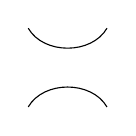
\begin{tikzpicture}[baseline={([yshift=-3pt]current bounding box.center)}]
    \draw (0,0) to [bend left=60] (1,0);
    \draw (0,1) to [bend right=60] (1,1);
\end{tikzpicture}%
}

% H pattern (horizontal connection)
\newcommand{\TLhorizontal}{%
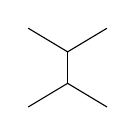
\begin{tikzpicture}[baseline={([yshift=-3pt]current bounding box.center)}]
    \draw (0,0) to (0.5,0.3) to (1,0);
    \draw (0,1) to (0.5,0.7) to (1,1);
    \draw (0.5,0.3) to (0.5,0.7);
\end{tikzpicture}%
}

% ============================================================
% Environment for Full Pentagon Diagram
% ============================================================
% Use the standalone file tex/figures/src/pentagon.tex for the full diagram
% or include inline with the patterns established above.

% ============================================================
% Environment for Full Hexagon Diagram
% ============================================================
% Use the standalone file tex/figures/src/hexagon.tex for the full diagram
% The hexagon.tex in literature/tex provides comprehensive examples.

% ============================================================
% END OF TIKZ STYLE LIBRARY
% ============================================================


% Configure listings for Julia
\lstset{
    language=Python,  % Julia syntax is close enough to Python
    basicstyle=\ttfamily\small,
    keywordstyle=\color{blue},
    commentstyle=\color{gray},
    stringstyle=\color{red},
    breaklines=true,
    frame=single,
    columns=fullflexible
}

% ============================================================
% Theorem Environments
% ============================================================
\theoremstyle{definition}
\newtheorem{definition}{Definition}[section]
\newtheorem{example}[definition]{Example}
\newtheorem{convention}[definition]{Convention}
\newtheorem{constraint}[definition]{Constraint}

\theoremstyle{plain}
\newtheorem{theorem}[definition]{Theorem}
\newtheorem{lemma}[definition]{Lemma}
\newtheorem{proposition}[definition]{Proposition}
\newtheorem{corollary}[definition]{Corollary}
\newtheorem{claim}[definition]{Claim}
\newtheorem{conjecture}[definition]{Conjecture}

\theoremstyle{remark}
\newtheorem{remark}[definition]{Remark}
\newtheorem{consequence}[definition]{Consequence}

% Custom environment for assumptions (with proper spacing for enumerated items)
\newenvironment{assumption}{%
  \par\medskip\noindent\textbf{Assumptions.}\par\nopagebreak\smallskip%
}{\par\medskip}

% ============================================================
% Custom Commands
% ============================================================
% Morphism notation (using Mor instead of Hom)
\DeclareMathOperator{\Mor}{Mor}
\DeclareMathOperator{\Hom}{Hom}
\DeclareMathOperator{\End}{End}
% \Tr already defined by physics package
\DeclareMathOperator{\Irr}{Irr}

% Category symbols
\newcommand{\catC}{\mathcal{C}}
\newcommand{\catH}{\mathcal{H}}
\newcommand{\catF}{\mathcal{F}}
\newcommand{\catO}{\mathcal{O}}

% Unit object
\newcommand{\one}{\mathbf{1}}

% Citation status markers
\newcommand{\unverified}{\texttt{[unverified]}}
\newcommand{\verified}{\texttt{[verified]}}
\newcommand{\original}{\texttt{[original]}}

% Citation block environment
\newenvironment{citationblock}{\par\noindent\textit{Reference:} }{\par}

% ============================================================
% Document Info
% ============================================================
\title{Microscopic Models for Mobile Anyons from Fusion Categories}
\author{Tobias J. Osborne}
\date{\today}

% ============================================================
% Document
% ============================================================
\begin{document}

\maketitle

\begin{abstract}
We develop a systematic framework for constructing microscopic lattice models describing mobile (itinerant) anyons arising from an arbitrary fusion category. Unlike existing models such as the golden chain where anyons are fixed at predetermined positions, our framework allows both the positions and number of anyons to fluctuate dynamically. Working in a first-quantised formalism on a one-dimensional chain with open boundary conditions, we construct Hilbert spaces that accommodate variable anyon number and anyon mobility, and define microscopic Hamiltonians for physically motivated scenarios. The framework is validated by reduction to known limiting cases including standard bosonic/fermionic systems and tightly-packed fusion chains.
\end{abstract}

\tableofcontents
\newpage

% ============================================================
% Introduction
% ============================================================
% introduction.tex
% Section 2: Introduction

\section{Introduction}
\label{sec:introduction}

\subsection{Why Mobile Anyons?}
\label{sec:why-mobile-anyons}

Anyonic particles---quasiparticle excitations obeying exotic exchange statistics that interpolate between bosonic and fermionic behaviour---have become central objects of study in condensed matter physics and quantum information theory. The mathematical framework of fusion categories provides a rigorous foundation for describing systems of anyons, encoding their fusion rules, braiding statistics, and algebraic structure in a unified formalism~\cite{Kitaev2006,ENO2005}.

Existing microscopic many-body models based on fusion categories, such as the celebrated golden chain~\cite{Feiguin2007}, describe systems where anyons occupy fixed positions on a lattice. In such models, the number of anyons is constant and their positions are predetermined---analogous to the tightly-packed Mott insulating phase in condensed matter systems. While these models have yielded profound insights into anyonic physics, including connections to conformal field theory at criticality, they represent only a special limiting case of the broader landscape of possible anyonic phases.

In realistic physical systems, however, particle number and position are typically dynamical degrees of freedom. Electrons in metals move freely through the lattice; ultracold atoms in optical lattices tunnel between sites; quasiparticles in quantum Hall systems can be created, annihilated, and transported. A complete understanding of anyonic matter requires extending the categorical framework to accommodate such \emph{mobile} or \emph{itinerant} anyons.

The motivation for developing microscopic models of mobile anyons is threefold:

\begin{enumerate}[label=(\roman*)]
    \item \textbf{Connection to realistic physics.} Physical systems supporting anyonic excitations---such as fractional quantum Hall states or topological superconductors---generically allow for variable anyon number and mobility. Microscopic models capturing these features would bridge the gap between abstract categorical data and experimentally accessible phenomena including transport, scattering, and thermodynamic properties.

    \item \textbf{Exploration of new phases.} Beyond the Mott-like limit of fixed anyons, one expects a rich phase diagram including dilute anyonic gases, anyonic superfluids, and intermediate correlated phases. The interplay between anyonic exchange statistics and spatial dynamics may give rise to novel collective phenomena without analogue in conventional bosonic or fermionic systems.

    \item \textbf{Recovery of known limits.} A consistent framework must reproduce well-understood special cases. When fusion rules are trivial ($X \otimes X = \one$), we should recover ordinary bosons or fermions depending on the braiding structure. For super-vector spaces (sVec), the construction should reduce exactly to fermionic Fock space with standard anticommutation relations. For dense configurations, we should recover the physics of the golden chain and related models.
\end{enumerate}

The present work addresses this gap by developing a systematic framework for constructing microscopic lattice models describing mobile anyons arising from an arbitrary fusion category. Working in a first-quantised formalism on a one-dimensional chain with open boundary conditions, we construct Hilbert spaces that accommodate variable anyon number and anyon mobility, and define microscopic Hamiltonians for physically motivated scenarios.

\subsection{Literature Gap}
\label{sec:literature-gap}

The theoretical study of anyonic systems has developed along two largely disjoint lines. On the mathematical side, the theory of fusion categories~\cite{ENO2005,EGNO2015} provides a complete algebraic framework for describing anyon types, their fusion rules, and braiding statistics. This framework is abstract and basis-independent, applicable to any system whose excitations form a fusion category. On the physical side, microscopic lattice models---most prominently the golden chain~\cite{Feiguin2007} and its generalisations---have demonstrated how to construct explicit Hamiltonians whose low-energy physics is governed by anyonic degrees of freedom.

However, these microscopic models invariably assume a \emph{dense} configuration: one anyon occupies each lattice site, and the Hilbert space is spanned by the different ways adjacent anyons can fuse. This corresponds to a Mott-insulating regime where particle number is maximal and fixed, and spatial dynamics are frozen out. The only degrees of freedom are the internal fusion channels---essentially, which superselection sector the system occupies locally.

Several important physical questions lie outside this dense limit:
\begin{itemize}
    \item \textbf{Dilute anyonic gases.} What is the ground state of a system with fewer anyons than sites? How do anyonic statistics affect spatial correlations in a dilute gas?
    \item \textbf{Hopping and transport.} If anyons can tunnel between sites, how does the interplay of mobility and exotic statistics manifest in transport properties?
    \item \textbf{Variable particle number.} Can we define pair-creation and annihilation processes consistent with fusion rules? What phases emerge when particle number fluctuates?
    \item \textbf{Interpolation to known limits.} A framework for mobile anyons should reduce to standard fermionic or bosonic physics when the fusion category is trivial (sVec or Vec respectively), providing a consistency check and physical intuition.
\end{itemize}

To our knowledge, no systematic framework exists for constructing microscopic lattice models of mobile anyons arising from a general fusion category. The present work aims to fill this gap.

\subsection{Contributions of This Work}
\label{sec:contributions}

This paper develops a systematic framework for mobile anyons on a one-dimensional lattice, making the following contributions:

\begin{enumerate}[label=(\arabic*)]
    \item \textbf{First-quantised Fock space construction.} We construct Hilbert spaces $\mathcal{H}_N^{(c)}$ for $N$ anyons with total charge $c$, built from morphism spaces of the underlying fusion category. The total Hilbert space $\mathcal{H} = \bigoplus_N \mathcal{H}_N$ accommodates variable particle number without invoking second-quantised creation/annihilation operators.

    \item \textbf{Configuration space formalism.} We define labelled configurations $(\mathbf{j}, \mathbf{k})$ specifying both positions and anyon types, with careful treatment of hard-core (at most one anyon per site) and soft-core (multiple occupancy allowed) constraints.

    \item \textbf{Local operator algebra.} We characterise the space of $k$-local operators---those acting nontrivially on at most $k$ consecutive sites---in terms of morphisms between tensor products of simple objects. This provides the building blocks for physically motivated Hamiltonians.

    \item \textbf{Explicit matrix elements.} For 2-local operators, we derive matrix element formulas in the fusion tree basis, expressing hopping, interaction, and braiding terms in terms of the category's F-symbols.

    \item \textbf{Recovery of standard limits.} We verify that when specialised to sVec (super-vector spaces), the construction reduces exactly to fermionic Fock space with the correct anticommutation relations and Jordan--Wigner structure.

    \item \textbf{Boundary conditions via module categories.} We show how module categories over $\mathcal{C}$ naturally encode boundary conditions, connecting the bulk categorical data to edge physics.
\end{enumerate}

% Placeholder for subsequent subsections
% \subsection{Paper Outline}
% \label{sec:paper-outline}


% ============================================================
% Part I: Preliminaries
% ============================================================
\part{Preliminaries}

% Section 3.1.1: Fusion Ring
% fusion_ring.tex
% LaTeX counterpart of docs/fusion_ring.md
% Section §3.1.1

\section{Fusion Ring}\label{sec:fusion-ring}

\begin{assumption}\label{ass:fusion-ring}
\begin{enumerate}[label=(A\arabic*)]
    \item Finite set of simple objects $\{X_i\}_{i=0}^{d_{\mathcal{C}}-1}$.
    \item Structure constants $N_{ab}^c \in \mathbb{Z}_{\ge 0}$ are associative and unital with unit $\mathbf{1}$.
\end{enumerate}
\end{assumption}

\subsection{Simple Objects}\label{subsec:simple-objects}

\begin{definition}[Simple object]\label{def:simple-object}
Let $\mathcal{C}$ be a fusion category over field $\mathbb{C}$. An object $X \in \mathcal{C}$ is \emph{simple} if it satisfies all three conditions:
\begin{enumerate}
    \item \textbf{Nonzero:} $X \neq 0$ (in the sense that $X$ is not the zero object).
    \item \textbf{Indecomposable:} If $X \cong Y \oplus Z$, then $Y = 0$ or $Z = 0$.
    \item \textbf{Schur:} $\End(X) \cong \mathbb{C}$ (all endomorphisms are scalar multiples of the identity).
\end{enumerate}
\end{definition}

\begin{consequence}\label{cons:semisimple-decomp}
By semisimplicity of fusion categories (Deligne's theorem), every object $A \in \mathcal{C}$ decomposes as a finite direct sum of simple objects:
\begin{equation}
    A \cong \bigoplus_{i \in I} X_i^{\oplus m_i}
\end{equation}
where $X_i$ are simple and $m_i \in \mathbb{Z}_{\ge 0}$ are multiplicities.
\end{consequence}

\begin{remark}
For our purposes, we work with fusion categories where the simple objects are \emph{distinguishable} by their labels: $\{X_0, X_1, \ldots, X_{d_{\mathcal{C}}-1}\}$ with $X_0 = \mathbf{1}$ (the tensor unit/vacuum).
\end{remark}

\begin{citationblock}
Etingof--Nikshych--Ostrik, \emph{Ann.\ Math.}\ \textbf{162} (2005), Theorem~2.7 \cite{ENO2005} \unverified
\end{citationblock}

\subsection{Fusion Ring Definition}\label{subsec:fusion-ring-def}

\begin{definition}[Fusion ring]\label{def:fusion-ring}
A \emph{fusion ring} is a finitely generated free abelian group $R = \bigoplus_{i \in I} \mathbb{Z} X_i$ with a ring structure satisfying:
\begin{enumerate}
    \item $X_0 = \mathbf{1}$ is the unit element.
    \item The product of basis elements satisfies
    \begin{equation}\label{eq:fusion-product}
        X_i X_j = \sum_{k\in I} N_{ij}^k X_k,
    \end{equation}
    where $N_{ij}^k \in \mathbb{Z}_{\ge 0}$ are the \emph{fusion coefficients} (or fusion multiplicities).
    \item There exists an involution $i \mapsto i^*$ such that
    \begin{equation}\label{eq:duality-condition}
        N_{ij}^0 = \delta_{i, j^*}.
    \end{equation}
\end{enumerate}
The involution gives duality: $X_i^* = X_{i^*}$. Associativity follows from the ring axioms:
\begin{equation}\label{eq:fusion-associativity}
    \sum_e N_{ij}^e N_{ek}^\ell = \sum_e N_{jk}^e N_{ie}^\ell \quad \text{for all } i, j, k, \ell \in I.
\end{equation}
\end{definition}

\begin{remark}
Fusion rings are generally \emph{not commutative}, i.e., $N_{ij}^k \neq N_{ji}^k$ in general.
\end{remark}

\begin{citationblock}
Etingof--Nikshych--Ostrik, \emph{Ann.\ Math.}\ \textbf{162} (2005), 581--642, Def.~3.1 \cite{ENO2005} \unverified
\end{citationblock}


% Section 3.1.2: Fusion Categories
% fusion_category.tex
% LaTeX counterpart of docs/fusion_category.md
% Section §3.1.2

\section{Fusion Categories}\label{sec:fusion-category}

\begin{assumption}\label{ass:fusion-category}
\begin{enumerate}[label=(A3.1.2.\arabic*)]
    \item Fusion ring $(R, \{X_i\}_{i\in I}, \mathbf{1})$ with $X_0 = \mathbf{1}$ and $N_{ij}^k \in \mathbb{Z}_{\ge 0}$ (Definition~\ref{def:fusion-ring}).
    \item Associator data $F$ (and, when present, braiding data $R$) satisfy the pentagon/hexagon equations.
\end{enumerate}
\end{assumption}

\begin{definition}[Fusion category]\label{def:fusion-category}
A \emph{fusion category} over an algebraically closed field $k$ (usually $k = \mathbb{C}$) is a $k$-linear, semisimple, rigid monoidal category
\begin{equation}
    (\mathcal{C}, \otimes, \mathbf{1})
\end{equation}
satisfying the following conditions:
\begin{enumerate}
    \item \textbf{Finiteness:} There are finitely many isomorphism classes of simple objects. Every object decomposes as a finite direct sum of simples.
    \item \textbf{Semisimplicity:} All morphism spaces $\Mor(X,Y)$ are finite-dimensional $k$-vector spaces, and the category is abelian and semisimple.
    \item \textbf{Rigidity:} Every object $X \in \mathcal{C}$ has a left and right dual $X^*$ with evaluation and coevaluation morphisms satisfying the rigidity axioms (Definition~\ref{def:rigidity-axioms}).
    \item \textbf{Simple unit:} The tensor unit $\mathbf{1}$ is simple: $\End(\mathbf{1}) \cong k$.
    \item \textbf{Finite $k$-linearity:} The monoidal structure is bilinear over $k$, and composition and tensor product of morphisms are $k$-linear.
\end{enumerate}
\end{definition}

\begin{definition}[Rigidity axioms]\label{def:rigidity-axioms}
For an object $X$ with dual $X^*$, the \emph{evaluation} $\mathrm{ev}_X: X^* \otimes X \to \mathbf{1}$ and \emph{coevaluation} $\mathrm{coev}_X: \mathbf{1} \to X \otimes X^*$ morphisms must satisfy the \emph{rigidity axioms} (zigzag identities):
\begin{equation}\label{eq:rigidity-left}
    (\mathrm{ev}_X \otimes \mathrm{id}_X) \circ (\mathrm{id}_{X^*} \otimes \mathrm{coev}_X) = \mathrm{id}_X
\end{equation}
\begin{equation}\label{eq:rigidity-right}
    (\mathrm{id}_{X^*} \otimes \mathrm{ev}_X) \circ (\mathrm{coev}_X \otimes \mathrm{id}_{X^*}) = \mathrm{id}_{X^*}
\end{equation}
Diagrammatically, these are the ``straightening'' of a bent string (cup followed by cap yields identity).
\end{definition}

\begin{definition}[Simple objects of a category]\label{def:irr}
For a fusion category $\mathcal{C}$, we denote by $\mathrm{Irr}(\mathcal{C})$ the set of isomorphism classes of simple objects. We write $[X] \in \mathrm{Irr}(\mathcal{C})$ for the isomorphism class containing simple object $X$.
\end{definition}

\begin{definition}[Quantum dimension]\label{def:quantum-dimension}
For a simple object $X$ in a fusion category $\mathcal{C}$, the \emph{quantum dimension} $d_X$ is defined via the categorical trace:
\begin{equation}
    d_X = \mathrm{tr}(\mathrm{id}_X) = \mathrm{ev}_X \circ (\mathrm{id}_{X^*} \otimes \mathrm{coev}_{X^*}) \circ \mathrm{coev}_X
\end{equation}
Diagrammatically, $d_X$ is the value of a closed loop labelled by $X$. For the tensor unit, $d_{\mathbf{1}} = 1$. The \emph{total dimension} of the category is $\mathrm{dim}(\mathcal{C}) = \sum_{X \in \mathrm{Irr}(\mathcal{C})} d_X^2$.
\end{definition}

\begin{remark}
Quantum dimensions satisfy $d_X d_Y = \sum_Z N_{XY}^Z d_Z$ (compatible with fusion rules) and $d_X = d_{X^*}$. For unitary categories, $d_X \geq 1$ with equality iff $X$ is invertible.
\end{remark}

\begin{definition}[Skeletal category]\label{def:skeletal}
A category is \emph{skeletal} if isomorphic objects are equal: $X \cong Y$ implies $X = Y$. Every category is equivalent to a skeletal one, and for fusion categories we often work with a skeletal representative where the simple objects are $\{X_0, X_1, \ldots, X_{d-1}\}$ with $X_0 = \mathbf{1}$.
\end{definition}

\begin{definition}[Grothendieck ring]\label{def:grothendieck-ring}
From any fusion category $\mathcal{C}$, we construct its \emph{Grothendieck ring} $K_0(\mathcal{C})$ by
\begin{equation}
    K_0(\mathcal{C}) = \bigoplus_{[X] \in \mathrm{Irr}(\mathcal{C})} \mathbb{Z} [X],
\end{equation}
with multiplication
\begin{equation}
    [X] \cdot [Y] = \sum_{Z} N_{XY}^{Z} [Z],
\end{equation}
where $N_{XY}^{Z} = \dim_k \Mor(X \otimes Y, Z)$ is the fusion multiplicity. The Grothendieck ring $K_0(\mathcal{C})$ is a fusion ring (Definition~\ref{def:fusion-ring}), establishing that \emph{fusion categories categorify fusion rings}.
\end{definition}

\begin{definition}[Braided fusion category]\label{def:braided-fusion-category}
If additionally $\mathcal{C}$ is equipped with a braiding (natural isomorphisms $c_{X,Y}: X \otimes Y \to Y \otimes X$ satisfying hexagon identities), we call $\mathcal{C}$ a \emph{braided fusion category}.
\end{definition}

\begin{citationblock}
Etingof--Gelaki--Nikshych--Ostrik, \emph{Tensor Categories}, AMS (2015), Ch.~4 and Ch.~8 \cite{EGNO2015} \unverified
\end{citationblock}

\subsection{F-Symbols and Pentagon Equation}

\begin{definition}[F-symbols]\label{def:f-symbols}
The \emph{associator} is a natural isomorphism
\begin{equation}
    \alpha_{a,b,c}: (a \otimes b) \otimes c \xrightarrow{\sim} a \otimes (b \otimes c)
\end{equation}
that satisfies the pentagon equation (Definition~\ref{def:pentagon}). In a skeletal category (Definition~\ref{def:skeletal}), the associator is determined by its matrix elements, the \emph{F-symbols}.

For simple objects $a,b,c,d$, the isomorphism decomposes into blocks indexed by intermediate fusion channels $e$ (for $(a \otimes b) \to e \to d$) and $f$ (for $(b \otimes c) \to f \to d$). The change of basis is given by the \emph{F-move}:
\begin{equation}\label{eq:f-move}
    \left| (a \otimes b) \otimes c \to d ; e, \alpha, \beta \right\rangle = \sum_{f, \mu, \nu} (F_{abc}^d)_{e, \alpha, \beta}^{f, \mu, \nu} \left| a \otimes (b \otimes c) \to d ; f, \mu, \nu \right\rangle
\end{equation}
where $\alpha, \beta, \mu, \nu$ are \emph{multiplicity indices}.
\end{definition}

\begin{remark}[Multiplicity indices]\label{rem:multiplicity-indices}
The indices $\alpha, \beta, \mu, \nu$ label basis vectors within fusion spaces when fusion multiplicities $N_{ab}^c > 1$. Specifically:
\begin{itemize}
    \item $\alpha \in \{1, \ldots, N_{ab}^e\}$ labels basis morphisms in $\Mor(a \otimes b, e)$
    \item $\beta \in \{1, \ldots, N_{ec}^d\}$ labels basis morphisms in $\Mor(e \otimes c, d)$
    \item $\mu \in \{1, \ldots, N_{bc}^f\}$ labels basis morphisms in $\Mor(b \otimes c, f)$
    \item $\nu \in \{1, \ldots, N_{af}^d\}$ labels basis morphisms in $\Mor(a \otimes f, d)$
\end{itemize}
For \emph{multiplicity-free} categories (where all $N_{ab}^c \in \{0,1\}$), these indices are trivial and can be suppressed.
\end{remark}

\begin{definition}[Pentagon equation]\label{def:pentagon}
The \emph{pentagon equation} ensures that the two paths to re-associate $((a \otimes b) \otimes c) \otimes d$ to $a \otimes (b \otimes (c \otimes d))$ coincide. In terms of F-symbols (suppressing multiplicity indices):
\begin{equation}\label{eq:pentagon}
    \sum_{k} (F_{a,b,c}^k)_e^l (F_{a,k,d}^p)_l^m (F_{b,c,d}^p)_k^n = (F_{a,b,n}^p)_e^m (F_{e,c,d}^m)_l^n
\end{equation}
This coherence condition is required for the fusion category to be well-defined.
\end{definition}

\subsection{R-Symbols and Hexagon Equations}

\begin{definition}[R-symbols]\label{def:r-symbols}
For a braided fusion category, the \emph{braiding isomorphism} $c_{a,b}: a \otimes b \to b \otimes a$ provides a natural way to permute tensor factors. For simple objects $a,b,c$, the braiding isomorphism is represented by its matrix elements, the \emph{R-symbols}.
\end{definition}

\begin{definition}[Hexagon equations]\label{def:hexagon}
The \emph{hexagon equations} are coherence conditions that relate the associator (F-symbols) and the braiding (R-symbols), ensuring consistency between re-associating and braiding operations. The first hexagon equation:
\begin{equation}\label{eq:hexagon}
    c_{a, b \otimes c} \circ (1_a \otimes c_{b,c}) = ((c_{a,b} \otimes 1_c) \circ F_{b,a,c} \circ (1_b \otimes c_{a,c})) \circ F_{a,c,b}^{-1}
\end{equation}
This equation (and its dual) ensures that braiding past a composite object can be decomposed consistently.
\end{definition}

\begin{citationblock}
Etingof--Gelaki--Nikshych--Ostrik, \emph{Tensor Categories}, AMS (2015), \S8.1--8.2 \cite{EGNO2015} \unverified
\end{citationblock}


% Section 3.1.3: Morphism Spaces
% morphism_spaces.tex
% LaTeX counterpart of docs/morphism_spaces.md
% Section §3.1.3

\section{Morphism Spaces and Multiplicities}\label{sec:morphism-spaces}

\begin{assumption}\label{ass:morphism-spaces}
\begin{enumerate}[label=(A3.1.3.\arabic*)]
    \item Fusion category $(\mathcal{C}, \otimes, \mathbf{1})$ over an algebraically closed field $k$ (Definition~\ref{def:fusion-category}).
    \item $\mathcal{C}$ is semisimple and $k$-linear, so all morphism spaces are finite-dimensional $k$-vector spaces.
\end{enumerate}
\end{assumption}

\begin{definition}[Morphism space]\label{def:morphism-space}
For any objects $A, B \in \mathcal{C}$,
\begin{equation}
    \Mor(A, B) := \Hom_{\mathcal{C}}(A, B)
\end{equation}
is a finite-dimensional $k$-vector space. If $A, B$ are simple, Schur's lemma implies $\dim \Mor(A, B) = \delta_{A, B}$.
\end{definition}

\begin{citationblock}
Etingof--Gelaki--Nikshych--Ostrik, \emph{Tensor Categories}, AMS (2015), \S4.2 \cite{EGNO2015} \unverified
\end{citationblock}

\begin{definition}[Fusion multiplicity space]\label{def:fusion-multiplicity-space}
For simple objects $X_a, X_b, X_c \in \mathrm{Irr}(\mathcal{C})$, the space
\begin{equation}
    \Mor(X_a \otimes X_b, X_c)
\end{equation}
has dimension $N_{ab}^c = \dim \Mor(X_a \otimes X_b, X_c) \in \mathbb{Z}_{\ge 0}$. A \emph{multiplicity basis} is any choice of morphisms
\begin{equation}
    f_{ab \to c}^{(\mu)} : X_a \otimes X_b \to X_c, \quad \mu = 1, \ldots, N_{ab}^c.
\end{equation}
No canonical choice exists; computations must remain basis-independent.
\end{definition}

\begin{claim}[Multiplicity-free simplification]\label{claim:mult-free}
In the multiplicity-free case ($N_{ab}^c \in \{0, 1\}$), each space $\Mor(X_a \otimes X_b, X_c)$ is either $\{0\}$ or a one-dimensional $k$-line. Basis dependence disappears, and $f_{ab \to c}^{(1)}$ can be chosen uniquely up to phase.
\end{claim}

\begin{remark}
Duals: $\Mor(\mathbf{1}, X_a \otimes X_b)$ is canonically dual to $\Mor(X_a^* \otimes X_b^*, \mathbf{1})$ via rigidity. Normalisation choices for evaluation/coevaluation maps must be consistent.
\end{remark}

\begin{remark}
Basis independence is essential for categorical definitions. Fusion-tree bases are admissible for computations (e.g., numerical evaluation of $F$-symbols) but must be removed from statements of definitions and theorems.
\end{remark}


% Section 3.1.6: Fusion Tree Basis
% fusion_tree_basis.tex
% Section §3.1.6: Fusion tree bases
% Discusses how fusion trees provide bases for morphism spaces

\section{Fusion Tree Basis}\label{sec:fusion-tree-basis}

\begin{assumption}\label{ass:fusion-tree-basis}
\begin{enumerate}[label=(A3.1.6.\arabic*)]
    \item Fusion category $(\mathcal{C}, \otimes, \mathbf{1})$ over $k = \mathbb{C}$ (Definition~\ref{def:fusion-category}).
    \item Simple objects $\{X_0, X_1, \ldots, X_{d-1}\}$ with $X_0 = \mathbf{1}$ (skeletal convention, Definition~\ref{def:skeletal}).
    \item Fusion multiplicities $N_{ab}^c = \dim \Mor(X_a \otimes X_b, X_c)$ (Definition~\ref{def:fusion-multiplicity-space}).
\end{enumerate}
\end{assumption}

\subsection{Fusion Trees as Diagrams}

\begin{definition}[Binary fusion tree]\label{def:binary-fusion-tree}
A \emph{binary fusion tree} with $n$ external legs (leaves) labelled by simple objects $a_1, \ldots, a_n$ and root labelled by $c$ is a planar binary tree where:
\begin{enumerate}
    \item Each leaf carries a label $a_i \in \mathrm{Irr}(\mathcal{C})$.
    \item Each internal edge carries an \emph{intermediate channel} label $e \in \mathrm{Irr}(\mathcal{C})$.
    \item Each trivalent vertex with incoming labels $x, y$ and outgoing label $z$ satisfies $N_{xy}^z \geq 1$ (the fusion is allowed).
    \item If $N_{xy}^z > 1$, the vertex additionally carries a \emph{multiplicity index} $\mu \in \{1, \ldots, N_{xy}^z\}$.
    \item The root edge carries the total charge $c$.
\end{enumerate}
\end{definition}

\begin{example}[Three-anyon fusion tree]
For three anyons $a_1, a_2, a_3$ fusing to total charge $c$, the \emph{left-associated} fusion tree corresponds to $((a_1 \otimes a_2) \otimes a_3) \to c$:
\begin{center}
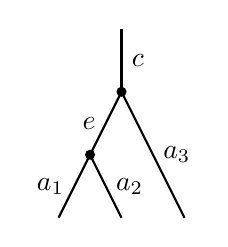
\begin{tikzpicture}[scale=0.8]
    % Left-associated tree: ((a1 ⊗ a2) ⊗ a3) → c
    \draw[thick] (0,0) -- (0.5,1) node[midway, left] {$a_1$};
    \draw[thick] (1,0) -- (0.5,1) node[midway, right] {$a_2$};
    \draw[thick] (0.5,1) -- (1,2) node[midway, left] {$e$};
    \draw[thick] (2,0) -- (1,2) node[midway, right] {$a_3$};
    \draw[thick] (1,2) -- (1,3) node[midway, right] {$c$};
    \filldraw (0.5,1) circle (2pt);
    \filldraw (1,2) circle (2pt);
\end{tikzpicture}
\end{center}
The intermediate channel $e$ ranges over all simple objects with $N_{a_1 a_2}^e \geq 1$ and $N_{e a_3}^c \geq 1$.
\end{example}

\subsection{Fusion Trees as Basis Vectors}

\begin{proposition}[Fusion tree basis]\label{prop:fusion-tree-basis}
The morphism space $\Mor(a_1 \otimes \cdots \otimes a_n, c)$ has a basis indexed by fusion trees with leaves $a_1, \ldots, a_n$ and root $c$. Specifically, for a fixed tree topology $T$ (e.g., left-associated), the basis vectors are indexed by:
\begin{enumerate}
    \item All valid assignments of intermediate channel labels to internal edges.
    \item All valid assignments of multiplicity indices to vertices.
\end{enumerate}
The dimension is
\begin{equation}
    \dim \Mor(a_1 \otimes \cdots \otimes a_n, c) = \sum_{\text{intermediate channels}} \prod_{\text{vertices } v} N_{x_v y_v}^{z_v}
\end{equation}
where the sum runs over all valid channel assignments and the product over all trivalent vertices.
\end{proposition}

\begin{example}[Dimension of $\Mor(a \otimes b \otimes c, d)$]
Using left-association:
\begin{equation}
    \dim \Mor(a \otimes b \otimes c, d) = \sum_{e \in \mathrm{Irr}(\mathcal{C})} N_{ab}^e \, N_{ec}^d.
\end{equation}
This equals $\sum_f N_{bc}^f N_{af}^d$ (right-association) by associativity of the Grothendieck ring.
\end{example}

\subsection{Change of Basis: F-Moves}

\begin{definition}[F-move as basis change]\label{def:f-move-basis}
The \emph{F-move} relates fusion tree bases corresponding to different association orders. For four anyons $a, b, c, d$, the F-symbol $(F_{abc}^d)_{e}^{f}$ (suppressing multiplicity indices) gives the overlap between:
\begin{itemize}
    \item Left-associated basis: $\ket{((a \otimes b) \otimes c) \to d; e}$ with intermediate channel $e$ in $(a \otimes b)$.
    \item Right-associated basis: $\ket{(a \otimes (b \otimes c)) \to d; f}$ with intermediate channel $f$ in $(b \otimes c)$.
\end{itemize}
The change of basis is:
\begin{equation}\label{eq:f-move-cob}
    \ket{(ab)c \to d; e} = \sum_{f} (F_{abc}^d)_{e}^{f} \ket{a(bc) \to d; f}.
\end{equation}
\end{definition}

\begin{remark}[Pentagon as consistency]
The pentagon equation (Definition~\ref{def:pentagon}) ensures that any sequence of F-moves relating two tree topologies yields the same result, regardless of the path taken through intermediate topologies. This is the defining coherence condition for monoidal categories.
\end{remark}

\subsection{Basis Independence}

\begin{convention}[Basis-independent formulations]\label{conv:basis-independence}
Physical quantities and categorical definitions should not depend on:
\begin{enumerate}
    \item The choice of tree topology (left-associated, right-associated, or other).
    \item The choice of multiplicity basis vectors $f_{ab \to c}^{(\mu)}$.
    \item Overall phase conventions for basis morphisms.
\end{enumerate}
Fusion tree bases are a \emph{computational tool}, not part of the categorical structure.
\end{convention}

\begin{remark}[When bases are necessary]
Explicit bases are required for:
\begin{itemize}
    \item Numerical computation of matrix elements (Section~\ref{sec:matrix-elements-2local}).
    \item Defining Hamiltonians in terms of F-symbols.
    \item Interface with TensorCategories.jl and similar software.
\end{itemize}
In such cases, one must verify that final results are basis-independent, or explicitly state which conventions are used.
\end{remark}

\begin{citationblock}
Kitaev, \emph{Anyons in an exactly solved model and beyond}, Ann.~Phys.~321 (2006), Appendix E \cite{Kitaev2006} \unverified
\end{citationblock}


% Section 3.1.8: Examples of Fusion Categories
% fusion_category_examples.tex
% LaTeX counterpart of docs/fusion_category_examples.md
% Section §3.1.8

\section{Examples of Fusion Categories}\label{sec:fusion-examples}

This section enumerates concrete fusion categories used in mobile anyon models. Each example specifies fusion rules, F-symbols, R-symbols (if braided), and the simple object count (rank).

\begin{assumption}\label{ass:fusion-examples}
\begin{enumerate}[label=(A3.1.8.\arabic*)]
    \item Fusion categories listed here are semisimple and rigid.
    \item Numerical F/R-symbols are computed via standard references (Kitaev, Rowell).
\end{enumerate}
\end{assumption}

%=============================================================
\subsection{Fibonacci Category (Multiplicity-Free)}\label{subsec:fibonacci}
%=============================================================

\textbf{Category:} $\mathcal{C}_{\mathrm{Fib}}$ \\
\textbf{Rank:} $d = 2$ \\
\textbf{Simple objects:} $\one = X_0$, $\tau = X_1$

\subsubsection{Fusion Rules}

\begin{center}
\begin{tabular}{c|cc}
$\otimes$ & $\one$ & $\tau$ \\
\hline
$\one$ & $\one$ & $\tau$ \\
$\tau$ & $\tau$ & $\one \oplus \tau$
\end{tabular}
\end{center}

\textbf{Multiplicities:} $N_{\tau\tau}^{\one} = N_{\tau\tau}^{\tau} = 1$ (multiplicity-free).

\subsubsection{Quantum Dimensions}

\begin{itemize}
    \item $d_{\one} = 1$
    \item $d_\tau = \phi = \frac{1+\sqrt{5}}{2}$ (golden ratio)
\end{itemize}

\subsubsection{F-Symbols (Associator)}

For the only nontrivial fusion channel $\tau \otimes \tau \to \one \oplus \tau$:
\begin{equation}
    F_{\tau,\tau,\tau}^\tau = \begin{pmatrix} \phi^{-1} & \phi^{-1/2} \\ \phi^{-1/2} & -\phi^{-1} \end{pmatrix}
\end{equation}
where rows/columns are indexed by the intermediate fusion channel $e \in \{\one, \tau\}$, and the matrix connects the two fusion orders: $(\tau \otimes \tau) \otimes \tau$ vs.\ $\tau \otimes (\tau \otimes \tau)$. This matrix is unitary: $F^\dagger F = I$.

\textbf{Numerical values:} $\phi^{-1} = \phi - 1 \approx 0.6180$, $\phi^{-1/2} \approx 0.7861$ \cite{Kitaev2006} \verified

\subsubsection{R-Symbols (Braiding)}

For the \emph{braided} Fibonacci category (adding R-symbols to the fusion category):
\begin{equation}
    R_{\tau,\tau}^{\one} = e^{4\pi i/5}, \qquad R_{\tau,\tau}^{\tau} = e^{-3\pi i/5}
\end{equation}
The topological spin (twist) of $\tau$ is $\theta_\tau = e^{4\pi i/5}$, corresponding to conformal weight $h_\tau = 2/5$. \verified

%=============================================================
\subsection{Ising Category (Multiplicity-Free)}\label{subsec:ising}
%=============================================================

\textbf{Category:} $\mathcal{C}_{\mathrm{Ising}}$ \\
\textbf{Rank:} $d = 3$ \\
\textbf{Simple objects:} $\one = X_0$, $\sigma = X_1$, $\psi = X_2$

\subsubsection{Fusion Rules}

\begin{center}
\begin{tabular}{c|ccc}
$\otimes$ & $\one$ & $\sigma$ & $\psi$ \\
\hline
$\one$ & $\one$ & $\sigma$ & $\psi$ \\
$\sigma$ & $\sigma$ & $\one \oplus \psi$ & $\sigma$ \\
$\psi$ & $\psi$ & $\sigma$ & $\one$
\end{tabular}
\end{center}

\textbf{Multiplicities:} All fusion coefficients are $0$ or $1$ (multiplicity-free).

\subsubsection{Quantum Dimensions}

\begin{itemize}
    \item $d_{\one} = 1$
    \item $d_\sigma = \sqrt{2}$
    \item $d_\psi = 1$
\end{itemize}

\subsubsection{F-Symbols}

Non-trivial associators exist for $\sigma \otimes \sigma \to \one \oplus \psi$:
\begin{equation}
    F_{\sigma,\sigma,\sigma}^\sigma = \frac{1}{\sqrt{2}} \begin{pmatrix} 1 & 1 \\ 1 & -1 \end{pmatrix}
\end{equation}
This is the Hadamard matrix, which is unitary. \verified

\subsubsection{R-Symbols}

For braided (modular) Ising category:
\begin{equation}
    R_{\sigma,\sigma}^{\one} = e^{i\pi/8}, \quad R_{\sigma,\sigma}^{\psi} = e^{-3i\pi/8}
\end{equation}
The topological spin of $\sigma$ is $\theta_\sigma = e^{i\pi/8}$. \verified

%=============================================================
\subsection{$\mathbb{Z}_N$ Categories (Pointed)}\label{subsec:zn}
%=============================================================

\textbf{Category:} $\mathcal{C}_{\mathbb{Z}_N}$ \\
\textbf{Rank:} $d = N$ \\
\textbf{Simple objects:} $X_0, X_1, \ldots, X_{N-1}$ (cyclic group)

\subsubsection{Fusion Rules}

\begin{equation}
    X_a \otimes X_b = X_{(a+b) \bmod N}
\end{equation}

\textbf{Multiplicities:} All $N_{ab}^c = 0$ or $1$ (multiplicity-free for standard abelian fusion).

\subsubsection{Quantum Dimensions}

$d_{X_a} = 1$ for all $a$. (For abelian/pointed categories, all objects are invertible and hence have quantum dimension $1$; see EGNO \S8.4 \cite{EGNO2015}.)

\subsubsection{F-Symbols}

For abelian (group-like) fusion, all nontrivial associators are trivial:
\begin{equation}
    F_{a,b,c}^e = 1
\end{equation}

\subsubsection{R-Symbols}

Braiding given by a 2-cocycle $\sigma(a, b) \in U(1)$:
\begin{equation}
    R_{a,b}^{a+b} = \sigma(a, b)
\end{equation}

\begin{example}[$\mathbb{Z}_2$ with fermionic statistics]
\begin{equation}
    R_{\mathrm{f}, \mathrm{f}}^{\one} = -1
\end{equation}
\end{example}

%=============================================================
\subsection{sVec Category (Fermionic)}\label{subsec:svec}
%=============================================================

\textbf{Category:} $\mathcal{C}_{\mathrm{sVec}}$ \\
\textbf{Rank:} $d = 2$ \\
\textbf{Simple objects:} $\one = X_0$ (boson), $\psi = X_1$ (fermion)

\subsubsection{Fusion Rules}

\begin{center}
\begin{tabular}{c|cc}
$\otimes$ & $\one$ & $\psi$ \\
\hline
$\one$ & $\one$ & $\psi$ \\
$\psi$ & $\psi$ & $\one$
\end{tabular}
\end{center}

\textbf{Multiplicities:} Multiplicity-free ($N_{\psi\psi}^{\one} = 1$).

\subsubsection{Quantum Dimensions}

\begin{itemize}
    \item $d_{\one} = 1$
    \item $d_\psi = 1$ (fermionic dimension)
\end{itemize}

\subsubsection{F-Symbols}

For fermionic fusion (super-case), the associator has an extra sign:
\begin{equation}
    F_{\psi,\psi,\psi}^{\one} = 1 \quad \text{(standard)}
\end{equation}
But crossing rules differ due to Fermi statistics.

\subsubsection{R-Symbols}

\begin{equation}
    R_{\psi,\psi}^{\one} = e^{i\pi} = -1
\end{equation}
(fermionic exchange is anticommuting; eigenvalue is $-1$).

%=============================================================
\subsection{Categories with Multiplicities}\label{subsec:multiplicity-examples}
%=============================================================

Most physically relevant fusion categories are multiplicity-free ($N_{ab}^c \in \{0,1\}$), but multiplicities arise in important examples.

\subsubsection{$SU(2)_k$ for $k \geq 3$}

\textbf{Category:} $\mathcal{C}_{SU(2)_k}$ (level-$k$ truncation of $SU(2)$ representations) \\
\textbf{Rank:} $d = k+1$ \\
\textbf{Simple objects:} $V_0, V_1, \ldots, V_k$ (spin-$j/2$ representations with $j = 0, 1, \ldots, k$)

\textbf{Fusion rules:} Truncated Clebsch--Gordan:
\begin{equation}
    V_a \otimes V_b = \bigoplus_{c = |a-b|}^{\min(a+b, 2k-a-b)} V_c
\end{equation}
where the sum runs in steps of $2$.

\textbf{Multiplicities:} For $k \geq 3$, we have $N_{ab}^c > 1$ in some cases. For instance, in $SU(2)_4$:
\begin{equation}
    V_2 \otimes V_2 = V_0 \oplus V_2 \oplus V_4
\end{equation}
is multiplicity-free, but higher levels exhibit multiplicities.

\begin{remark}[Other multiplicity examples]
Categories with multiplicities include:
\begin{itemize}
    \item Haagerup categories $\mathcal{H}_1, \mathcal{H}_2, \mathcal{H}_3$ (exotic fusion categories)
    \item Tambara--Yamagami categories for non-abelian groups
    \item Representation categories of quantum groups at roots of unity
\end{itemize}
The general framework developed in this paper handles multiplicities via multiplicity indices (Remark~\ref{rem:multiplicity-indices}).
\end{remark}

%=============================================================
\subsection{Summary Table}\label{subsec:examples-summary}
%=============================================================

\begin{table}[h]
\centering
\begin{tabular}{lccccl}
\toprule
\textbf{Category} & \textbf{Rank} & \textbf{Mult-Free?} & \textbf{Braided?} & \textbf{Modular?} & \textbf{Status} \\
\midrule
Fibonacci & 2 & $\checkmark$ & $\checkmark$ & $\checkmark$ & Implemented \\
Ising & 3 & $\checkmark$ & $\checkmark$ & $\checkmark$ & Implemented \\
$\mathbb{Z}_N$ & $N$ & $\checkmark$ & $\checkmark$ & $\times$ & Template \\
sVec & 2 & $\checkmark$ & $\checkmark$ & $\times$ & Fermionic \\
$SU(2)_k$ & $k+1$ & $\times$ (for $k \geq 3$) & $\checkmark$ & $\checkmark$ & Reference \\
\bottomrule
\end{tabular}
\caption{Summary of fusion category examples.}
\label{tab:examples-summary}
\end{table}

\begin{remark}
\textbf{Unverified:} All F/R-symbol values marked \unverified\ pending HITL review against literature.
\end{remark}

\begin{remark}
\textbf{Not exhaustive:} Other fusion categories (e.g., Haagerup, $SU(2)_k$, Tambara--Yamagami) can be added as needed. Note: Potts models and Virasoro algebras are related CFT structures but are not themselves fusion categories.
\end{remark}


% Section 3.1a: Temperley-Lieb Categories
% temperley_lieb.tex
% LaTeX counterpart of docs/temperley_lieb.md
% Section §3.1a

\section{Temperley--Lieb Categories}\label{sec:temperley-lieb}

\begin{assumption}\label{ass:temperley-lieb}
\begin{enumerate}[label=(A\arabic*)]
    \item Loop fugacity $n = q + q^{-1}$ for quantum parameter $q$.
    \item At roots of unity $q = e^{i\pi/p}$, the category truncates to finitely many simples.
    \item Standard normalisation: loop evaluates to $\delta = -[2]_q$.
\end{enumerate}
\end{assumption}

\subsection{Overview}

The \emph{Temperley--Lieb (TL) category} is a fundamental example connecting fusion categories to statistical mechanics, loop models, and conformal field theory. TL categories provide:
\begin{enumerate}
    \item A continuous interpolation between solvable models via the loop fugacity parameter.
    \item Concrete realisations of Fibonacci ($q = e^{i\pi/5}$) and Ising ($q = e^{i\pi/4}$) anyons.
    \item Direct connection to critical phenomena and CFT via the central charge formula.
\end{enumerate}

\subsection{Loop Fugacity Parametrisation}

The TL category is parametrised by the \emph{loop fugacity} $n$, related to the quantum parameter $q$ by:
\begin{equation}\label{eq:loop-fugacity}
    n = q + q^{-1} = 2\cos\theta, \qquad q = e^{i\theta}.
\end{equation}

\begin{example}[Key values of loop fugacity]
\begin{center}
\begin{tabular}{@{}lll@{}}
\toprule
$p$ (for $q = e^{i\pi/p}$) & $n = 2\cos(\pi/p)$ & Physical model \\
\midrule
$p = 3$ & $n = 1$ & Percolation \\
$p = 4$ & $n = \sqrt{2}$ & Ising ($\sigma$-anyon) \\
$p = 5$ & $n = \phi = \frac{1+\sqrt{5}}{2}$ & Fibonacci ($\tau$-anyon) \\
$p = 6$ & $n = \sqrt{3}$ & 3-state Potts \\
$p \to \infty$ & $n \to 2$ & Free fermion \\
\bottomrule
\end{tabular}
\end{center}
\end{example}

At roots of unity, the representation theory truncates, yielding \emph{modular tensor categories} with finitely many simple objects.

\subsection{Quantum Numbers}

\begin{definition}[Quantum integer]\label{def:quantum-integer}
For $q = e^{i\pi/p}$, the \emph{quantum integer} is:
\begin{equation}\label{eq:quantum-integer}
    [n]_q = \frac{q^n - q^{-n}}{q - q^{-1}} = \frac{\sin(n\pi/p)}{\sin(\pi/p)}.
\end{equation}
\end{definition}

\begin{definition}[Quantum factorial and binomial]\label{def:quantum-factorial}
The \emph{quantum factorial} and \emph{quantum binomial} are:
\begin{equation}
    [n]!_q = [1]_q [2]_q \cdots [n]_q, \qquad \binom{n}{k}_q = \frac{[n]!_q}{[k]!_q [n-k]!_q}.
\end{equation}
\end{definition}

\begin{remark}
At roots of unity, $[p-1]_q = 0$, causing the truncation of the representation theory.
\end{remark}

\subsection{Simple Objects and Fusion Rules}

At generic $q$, the TL category has infinitely many simple objects labelled by half-integers $j \in \{0, \frac{1}{2}, 1, \frac{3}{2}, \ldots\}$, corresponding to spins in the representation theory of $U_q(\mathfrak{sl}_2)$.

At roots of unity $q = e^{i\pi/p}$, the category \emph{truncates} to:
\begin{equation}\label{eq:tl-simples}
    j \in \left\{0, \frac{1}{2}, 1, \ldots, \frac{p-2}{2}\right\}.
\end{equation}

\begin{definition}[TL fusion rules]\label{def:tl-fusion}
The fusion rules are the $SU(2)_q$ rules with truncation:
\begin{equation}\label{eq:tl-fusion-rule}
    j_1 \otimes j_2 = \bigoplus_{j = |j_1 - j_2|}^{\min(j_1 + j_2, p-2-j_1-j_2)} j.
\end{equation}
\end{definition}

\subsection{Connection to Key Examples}

\begin{example}[Fibonacci anyons, $p = 5$]
Two simple objects $\{\one, \tau\}$ with $\tau \otimes \tau = \one \oplus \tau$.
\end{example}

\begin{example}[Ising anyons, $p = 4$]
Three simple objects $\{\one, \sigma, \psi\}$ with:
\begin{align}
    \sigma \otimes \sigma &= \one \oplus \psi, \\
    \psi \otimes \psi &= \one, \\
    \sigma \otimes \psi &= \sigma.
\end{align}
\end{example}

\subsection{Critical Behaviour}

\begin{theorem}[Central charge]\label{thm:tl-central-charge}
At $q = e^{i\pi/p}$, the TL algebra describes critical points with central charge:
\begin{equation}\label{eq:central-charge}
    c = 1 - \frac{6(p-1)^2}{p}.
\end{equation}
This connects TL categories to minimal model CFTs $\mathcal{M}(p, p-1)$.
\end{theorem}

\begin{citationblock}
Kauffman--Lins, \emph{Temperley--Lieb Recoupling Theory} (1994) \unverified;
Jones, \emph{Inventiones Math.}\ \textbf{72} (1983), 1--25 \unverified
\end{citationblock}


% Section 3.2: Fock Space
% fock_space.tex
% LaTeX counterpart of docs/fock_space.md
% Section §3.2

\section{Fock Space Perspective (First Quantisation)}\label{sec:fock-space}

\begin{assumption}\label{ass:fock-space}
\begin{enumerate}[label=(A3.2.\arabic*)]
    \item First-quantised formalism only (no $a^\dagger, a$).
    \item Fock space is a direct sum of fixed-number sectors.
\end{enumerate}
\end{assumption}

\subsection{Standard Fock Space}\label{subsec:standard-fock}

\begin{definition}[Fock space]\label{def:fock-space}
The \emph{Fock space} $\mathcal{F}$ is the direct sum of $N$-particle Hilbert spaces $\mathcal{H}_N$ for all possible particle numbers $N \ge 0$:
\begin{equation}\label{eq:fock-space}
    \mathcal{F} = \bigoplus_{N=0}^{\infty} \mathcal{H}_N = \mathcal{H}_0 \oplus \mathcal{H}_1 \oplus \mathcal{H}_2 \oplus \cdots
\end{equation}
where $\mathcal{H}_0 \cong \mathbb{C}$ is the vacuum sector spanned by the vacuum state $|\Omega\rangle$.
\end{definition}

\begin{remark}
In this first-quantised approach, a state $|\Psi\rangle \in \mathcal{F}$ is a sequence of wavefunctions (or categorical states) $|\Psi\rangle = (\psi_0, \psi_1, \psi_2, \ldots)$, where $\psi_N \in \mathcal{H}_N$ is the projection of the state onto the $N$-particle sector.
\end{remark}

\begin{constraint}
We strictly avoid the use of second-quantised creation/annihilation operators ($a_i^\dagger, a_i$) as fundamental building blocks. While convenient for bosons/fermions, they obscure the categorical data (braiding, fusion) essential for anyons.
\end{constraint}

\subsection{Direct Sum as ``OR Quantifier''}\label{subsec:direct-sum}

The direct sum ($\oplus$) operation represents a logical ``OR'' or superposition of different particle number sectors.

\begin{itemize}
    \item A state in $\mathcal{H}_1 \oplus \mathcal{H}_2$ describes a system that is in a superposition of having 1 particle \textbf{OR} 2 particles.
    \item This contrasts with the tensor product (see \S\ref{subsec:tensor-product-fock}).
\end{itemize}

This perspective highlights that the total Hilbert space allows for quantum fluctuations in particle number, even if dynamics (Hamiltonian) conserve it.

\subsection{Tensor Product as ``AND Quantifier''}\label{subsec:tensor-product-fock}

The tensor product ($\otimes$) operation represents a logical ``AND'' or composition of subsystems.

\begin{itemize}
    \item Within a fixed $N$-particle sector $\mathcal{H}_N$, the structure involves tensor products of single-particle spaces (or local site spaces):
    \begin{equation}
        \mathcal{H}_N \sim \mathcal{H}_{\mathrm{loc}} \otimes \cdots \otimes \mathcal{H}_{\mathrm{loc}} \quad \text{(schematically)}
    \end{equation}
    \item A state $|\phi\rangle \otimes |\chi\rangle$ describes a system where part A is in state $\phi$ \textbf{AND} part B is in state $\chi$.
\end{itemize}

\begin{remark}[Anyonic nuance]
For anyons, $\mathcal{H}_N$ is not a simple tensor product of single-particle spaces due to fusion constraints (fusion spaces are not product spaces). However, the \emph{ambient} space in which $\mathcal{H}_N$ is embedded (before fusion constraints) often has a tensor product structure (e.g., sites on a lattice).
\end{remark}

\subsection{First-Quantised Operators}\label{subsec:first-quant-ops}

\begin{definition}[Operator on Fock space]\label{def:fock-operator}
An operator $\hat{O} : \mathcal{F} \to \mathcal{F}$ is defined by its action on each sector $\mathcal{H}_N$ and maps between sectors. It can be represented as a matrix of operators $\hat{O}_{MN} : \mathcal{H}_N \to \mathcal{H}_M$.
\end{definition}

\begin{definition}[Number-conserving operator]\label{def:number-conserving}
An operator $\hat{H}$ is \emph{number-conserving} if it maps each sector $\mathcal{H}_N$ to itself ($\hat{H}_{MN} = 0$ for $M \neq N$). It decomposes as a direct sum of operators acting on fixed-number sectors:
\begin{equation}
    \hat{H} = \bigoplus_{N=0}^{\infty} \hat{H}_N
\end{equation}
where $\hat{H}_N : \mathcal{H}_N \to \mathcal{H}_N$.
\end{definition}

\begin{example}
The Hamiltonian for mobile anyons is typically number-conserving (unless studying source terms), so we construct it by defining a sequence of Hamiltonians $H_N$ for each $N$-anyon configuration space.
\end{example}

\subsection{Summary}

\begin{center}
\begin{tabular}{llll}
\toprule
\textbf{Structure} & \textbf{Symbol} & \textbf{Interpretation} & \textbf{Logical Equiv.} \\
\midrule
Direct Sum & $\oplus$ & Superposition of sectors & \textbf{OR} \\
Tensor Product & $\otimes$ & Composition of parts & \textbf{AND} \\
Fock Space & $\mathcal{F}$ & $\bigoplus_N \mathcal{H}_N$ & Variable particle number \\
Operator & $\hat{O}$ & $\bigoplus_N \hat{O}_N$ (if conserved) & Collection of $N$-particle ops \\
\bottomrule
\end{tabular}
\end{center}


% Section 3.3: QM for Lattice Models
% qm_lattice.tex
% LaTeX counterpart of docs/qm_lattice.md
% Section §3.3

\section{Quantum Mechanics for Lattice Models}\label{sec:qm-lattice}

\begin{assumption}\label{ass:qm-lattice}
\begin{enumerate}[label=(A3.3.\arabic*)]
    \item All Hilbert spaces are finite-dimensional.
    \item Hamiltonians are Hermitian.
\end{enumerate}
\end{assumption}

\subsection{Hilbert Spaces, States, Observables}\label{subsec:hilbert-basics}

\begin{definition}[Hilbert space]\label{def:hilbert-space}
A \emph{Hilbert space} $\mathcal{H}$ is a complex vector space equipped with an inner product $\langle \cdot | \cdot \rangle : \mathcal{H} \times \mathcal{H} \to \mathbb{C}$ that is complete with respect to the induced norm. In this work, all Hilbert spaces are finite-dimensional.
\end{definition}

\begin{definition}[State]\label{def:state}
A \emph{state} is a nonzero vector $|\psi\rangle \in \mathcal{H}$. Two states are physically equivalent if they differ by a nonzero scalar. Normalised states satisfy $\langle\psi|\psi\rangle = 1$.
\end{definition}

\begin{definition}[Observable]\label{def:observable}
An \emph{observable} is a Hermitian operator $A : \mathcal{H} \to \mathcal{H}$, i.e., $A = A^\dagger$ where $\langle \phi | A \psi \rangle = \langle A\phi | \psi \rangle$ for all $|\phi\rangle, |\psi\rangle$.
\end{definition}

\subsection{Hamiltonians for Lattice Systems}\label{subsec:hamiltonians}

\begin{definition}[Hamiltonian]\label{def:hamiltonian}
A \emph{Hamiltonian} is a Hermitian operator $H : \mathcal{H} \to \mathcal{H}$ representing the total energy of the system.
\end{definition}

\begin{definition}[Local Hamiltonian]\label{def:local-hamiltonian}
A Hamiltonian $H$ is \emph{local} if it decomposes as a sum of terms, each acting nontrivially on a bounded number of sites:
\begin{equation}
    H = \sum_j h_j
\end{equation}
where each $h_j$ acts on sites in a neighbourhood of $j$.
\end{definition}

\begin{definition}[Nearest-neighbour Hamiltonian]\label{def:nn-hamiltonian}
A Hamiltonian is \emph{nearest-neighbour} if each term $h_j$ acts nontrivially only on sites $j$ and $j+1$.
\end{definition}

\subsection{Ground States, Spectrum, Partition Function}\label{subsec:spectrum}

\begin{definition}[Spectrum]\label{def:spectrum}
The \emph{spectrum} of $H$ is the set of eigenvalues $\{E_0, E_1, \ldots\}$ ordered so that $E_0 \leq E_1 \leq \cdots$.
\end{definition}

\begin{definition}[Ground state]\label{def:ground-state}
A \emph{ground state} is an eigenvector of $H$ with eigenvalue $E_0$ (the minimum eigenvalue).
\end{definition}

\begin{definition}[Spectral gap]\label{def:spectral-gap}
The \emph{spectral gap} is $\Delta = E_1 - E_0$.
\end{definition}

\begin{definition}[Partition function]\label{def:partition-function}
The \emph{partition function} at inverse temperature $\beta$ is
\begin{equation}
    Z(\beta) = \Tr(e^{-\beta H}) = \sum_n e^{-\beta E_n}
\end{equation}
\end{definition}

\subsection{Tensor Product Structure}\label{subsec:tensor-product}

\begin{definition}[Tensor product of Hilbert spaces]\label{def:tensor-hilbert}
Given Hilbert spaces $\mathcal{H}_1, \mathcal{H}_2$, the \emph{tensor product} $\mathcal{H}_1 \otimes \mathcal{H}_2$ is a Hilbert space with:
\begin{itemize}
    \item $\dim(\mathcal{H}_1 \otimes \mathcal{H}_2) = \dim(\mathcal{H}_1) \cdot \dim(\mathcal{H}_2)$
    \item Basis: $\{|i\rangle \otimes |j\rangle\}$ for bases $\{|i\rangle\}$ of $\mathcal{H}_1$ and $\{|j\rangle\}$ of $\mathcal{H}_2$
\end{itemize}
\end{definition}

\begin{definition}[Multi-site Hilbert space]\label{def:multi-site-hilbert}
For $n$ sites with local Hilbert space $\mathcal{H}_{\mathrm{loc}}$ of dimension $d$, the total Hilbert space is
\begin{equation}
    \mathcal{H}_{\mathrm{total}} = \bigotimes_{j=1}^{n} \mathcal{H}_{\mathrm{loc}} \cong \mathbb{C}^{d^n}
\end{equation}
\end{definition}

\begin{remark}
The tensor product represents the ``AND quantifier'': a state in $\mathcal{H}_1 \otimes \mathcal{H}_2$ describes a system where both subsystem 1 AND subsystem 2 exist simultaneously. Cf.\ \S\ref{sec:fock-space}.
\end{remark}

\subsection{Summary}

\begin{center}
\begin{tabular}{lll}
\toprule
\textbf{Concept} & \textbf{Symbol} & \textbf{Definition} \\
\midrule
Hilbert space & $\mathcal{H}$ & Finite-dim complex inner product space \\
State & $|\psi\rangle$ & Nonzero vector in $\mathcal{H}$ \\
Observable & $A$ & Hermitian operator \\
Hamiltonian & $H$ & Hermitian operator (energy) \\
Ground state & $|\psi_0\rangle$ & Eigenvector with minimal eigenvalue \\
Partition function & $Z(\beta)$ & $\Tr(e^{-\beta H})$ \\
Tensor product & $\otimes$ & ``AND quantifier'' for composite systems \\
\bottomrule
\end{tabular}
\end{center}


% Section 3.4: Lattice Geometry
% lattice.tex
% LaTeX counterpart of docs/lattice.md
% Section §3.4

\section{Lattice Geometry}\label{sec:lattice}

\begin{assumption}\label{ass:lattice}
\begin{enumerate}[label=(A3.4.\arabic*)]
    \item Spatial dimension is 1.
    \item Open boundary conditions (no PBCs).
    \item Finite number of sites.
\end{enumerate}
\end{assumption}

\subsection{One-Dimensional Chain}\label{subsec:1d-chain}

\begin{definition}[Lattice]\label{def:lattice}
A \emph{lattice} $\Lambda$ is a finite set of sites. In this work:
\begin{equation}
    \Lambda = \{0, 1, 2, \ldots, n-1\}
\end{equation}
where $n = |\Lambda|$ is the number of sites.
\end{definition}

\begin{remark}
We use 0-based indexing for sites to align with physical position $x_j = \epsilon \cdot j$.
\end{remark}

\begin{definition}[Neighbour relation]\label{def:neighbour}
Sites $i$ and $j$ are \emph{neighbours} if $|i - j| = 1$. We write $i \sim j$.
\end{definition}

\begin{definition}[Boundary sites]\label{def:boundary}
The \emph{boundary} of $\Lambda$ consists of sites $0$ and $n-1$. The \emph{bulk} consists of sites $\{1, \ldots, n-2\}$.
\end{definition}

\subsection{Lattice Spacing and Physical Position}\label{subsec:spacing}

\begin{definition}[Physical length]\label{def:physical-length}
The \emph{physical length} of the system is $L > 0$.
\end{definition}

\begin{definition}[Lattice spacing]\label{def:lattice-spacing}
The \emph{lattice spacing} is
\begin{equation}
    \epsilon = \frac{L}{n}
\end{equation}
\end{definition}

\begin{definition}[Physical position]\label{def:physical-position}
The \emph{physical position} of site $j$ is
\begin{equation}
    x_j = \epsilon \cdot j = \frac{L \cdot j}{n}
\end{equation}
so that $x_0 = 0$ and $x_{n-1} = L(1 - 1/n) < L$.
\end{definition}

\begin{convention}
Where convenient, we set $\epsilon = 1$ (equivalently, $L = n$), so that site index equals physical position.
\end{convention}

\subsection{Open Boundary Conditions}\label{subsec:obc}

\begin{definition}[Open boundary conditions]\label{def:obc}
A system has \emph{open boundary conditions} (OBC) if:
\begin{enumerate}
    \item The lattice is a finite chain with distinct endpoints
    \item Site 0 has only one neighbour (site 1)
    \item Site $n-1$ has only one neighbour (site $n-2$)
\end{enumerate}
\end{definition}

\begin{remark}
This contrasts with \emph{periodic boundary conditions} (PBC) where site $n-1$ is also a neighbour of site 0. We exclude PBCs in this work (Assumption~A3.4.2).
\end{remark}

\begin{remark}
OBC implies:
\begin{itemize}
    \item No topological ground state degeneracy from nontrivial cycles
    \item Edge effects may be present
    \item Total charge is well-defined without ambiguity from winding
\end{itemize}
\end{remark}

\subsection{Local Hilbert Spaces}\label{subsec:local-hilbert}

\begin{definition}[Local Hilbert space]\label{def:local-hilbert}
Each site $j \in \Lambda$ carries a \emph{local Hilbert space} $\mathcal{H}_j$. For identical sites:
\begin{equation}
    \mathcal{H}_j \cong \mathcal{H}_{\mathrm{loc}} \quad \forall j
\end{equation}
\end{definition}

\begin{definition}[Local dimension]\label{def:local-dim}
The \emph{local dimension} is $d_{\mathrm{loc}} = \dim(\mathcal{H}_{\mathrm{loc}})$.
\end{definition}

\begin{definition}[Total Hilbert space]\label{def:total-hilbert-lattice}
The \emph{total Hilbert space} for the lattice is
\begin{equation}
    \mathcal{H}_{\mathrm{total}} = \bigotimes_{j=0}^{n-1} \mathcal{H}_j \cong \mathbb{C}^{d^n}
\end{equation}
\end{definition}

\begin{remark}
For mobile anyons, the local Hilbert space structure is more subtle---see \S\ref{sec:hilbert-space}. The ``local dimension'' depends on the occupation at that site.
\end{remark}

\subsection{Summary}

\begin{center}
\begin{tabular}{lll}
\toprule
\textbf{Concept} & \textbf{Symbol} & \textbf{Value/Definition} \\
\midrule
Number of sites & $n$ & $|\Lambda|$ \\
Site indices & $j$ & $0, 1, \ldots, n-1$ \\
Physical length & $L$ & System size \\
Lattice spacing & $\epsilon$ & $L/n$ \\
Physical position & $x_j$ & $\epsilon \cdot j$ \\
Local Hilbert space & $\mathcal{H}_j$ & Space at site $j$ \\
Local dimension & $d_{\mathrm{loc}}$ & $\dim(\mathcal{H}_{\mathrm{loc}})$ \\
Total dimension & --- & $d^n$ \\
\bottomrule
\end{tabular}
\end{center}

\subsection{Notation Conventions}

Throughout this project:
\begin{itemize}
    \item Sites are \textbf{0-indexed}: $j \in \{0, 1, \ldots, n-1\}$
    \item Boundary conditions are \textbf{open} (OBC)
    \item Default: $\epsilon = 1$ unless stated otherwise
    \item Tensor products are ordered left-to-right: $\mathcal{H}_0 \otimes \mathcal{H}_1 \otimes \cdots \otimes \mathcal{H}_{n-1}$
\end{itemize}


% ============================================================
% Part II: Hilbert Space for Mobile Anyons
% ============================================================
\part{Hilbert Space for Mobile Anyons}

% Section 4.1: Configuration Space
% config_space.tex
% LaTeX counterpart of docs/config_space.md
% Section §4.1

\section{Classical Configuration Space}\label{sec:config-space}

\begin{assumption}\label{ass:config-space}
\begin{enumerate}[label=(A4.1.\arabic*)]
    \item Fusion category $\mathcal{C}$ with simples $\{X_0, X_1, \ldots, X_{d-1}\}$ where $X_0 = \mathbf{1}$.
    \item Lattice $\Lambda = \{0, \ldots, n-1\}$ with OBC.
\end{enumerate}
\end{assumption}

\subsection{Anyon Positions}\label{subsec:anyon-positions}

\begin{definition}[Configuration]\label{def:configuration}
A \emph{configuration} of $N$ anyons is a tuple
\begin{equation}
    \mathbf{j} = (j_1, j_2, \ldots, j_N) \in \Lambda^N
\end{equation}
satisfying $0 \leq j_1 \leq j_2 \leq \cdots \leq j_N \leq n-1$.
\end{definition}

\begin{remark}
The ordering $j_1 \leq \cdots \leq j_N$ reflects indistinguishability up to exchange. Distinct orderings related by permutation represent the same physical configuration.
\end{remark}

\subsection{Anyon Labels}\label{subsec:anyon-labels}

\begin{definition}[Labelled configuration]\label{def:labelled-config}
A \emph{labelled configuration} is a pair $(\mathbf{j}, \mathbf{k})$ where:
\begin{itemize}
    \item $\mathbf{j} = (j_1, \ldots, j_N)$ is a configuration
    \item $\mathbf{k} = (k_1, \ldots, k_N)$ with $k_m \in \{1, \ldots, d-1\}$ labels the anyon type at site $j_m$
\end{itemize}
\end{definition}

\begin{convention}
Label $0$ denotes vacuum (no anyon). Labels $1, \ldots, d-1$ denote the nontrivial simple objects $X_1, \ldots, X_{d-1}$.
\end{convention}

\subsection{Configuration Space}\label{subsec:config-space-def}

\begin{definition}[$N$-anyon configuration space]\label{def:n-config-space}
\begin{equation}
    \mathrm{Conf}_N = \{(\mathbf{j}, \mathbf{k}) : \mathbf{j} \in \Lambda^N \text{ ordered}, \, k_m \in \{1,\ldots,d-1\}\}
\end{equation}
\end{definition}

\begin{definition}[Hard-core configuration space]\label{def:hc-config-space}
With hard-core constraint:
\begin{equation}
    \mathrm{Conf}_N^{\mathrm{HC}} = \{(\mathbf{j}, \mathbf{k}) \in \mathrm{Conf}_N : j_1 < j_2 < \cdots < j_N\}
\end{equation}
\end{definition}

\begin{claim}\label{claim:config-count}
$|\mathrm{Conf}_N^{\mathrm{HC}}| = \binom{n}{N}(d-1)^N$.
\end{claim}

\subsection{Mixed Character}\label{subsec:mixed-character}

\begin{remark}
Configurations have mixed identical/distinguishable character:
\begin{itemize}
    \item Anyons with \emph{same label} $k_i = k_j$ are identical
    \item Anyons with \emph{different labels} $k_i \neq k_j$ are distinguishable
\end{itemize}
This is handled by the morphism space structure in \S\ref{sec:hilbert-space}.
\end{remark}


% Section 4.2: Hilbert Space
% hilbert_space.tex
% LaTeX counterpart of docs/hilbert_space.md
% Section §4.2

\section{Hilbert Space for Mobile Anyons}\label{sec:hilbert-space}

\begin{assumption}\label{ass:hilbert-space}
\begin{enumerate}[label=(A4.2.\arabic*)]
    \item Fusion category $\mathcal{C}$ with unit $\mathbf{1}$ and simples $X_0=\mathbf{1}, X_1, \ldots, X_{d-1}$.
    \item $n$ lattice sites, OBC.
\end{enumerate}
\end{assumption}

\subsection{Morphism Spaces}\label{subsec:mor-spaces-hilbert}

\begin{definition}[Morphism space]\label{def:mor-space-hilbert}
For objects $A, B \in \mathcal{C}$:
\begin{equation}
    \Mor(A, B) = \Hom_{\mathcal{C}}(A, B)
\end{equation}
This is a finite-dimensional complex vector space with $\dim \Mor(A,B) = \delta_{A,B}$ for simple $A, B$ (in the multiplicity-free case).
\end{definition}

\begin{remark}
With multiplicity: $\dim \Mor(X_a \otimes X_b, X_c) = N_{ab}^c$.
\end{remark}

\subsection{$N$-Anyon Sector with Definite Charge}\label{subsec:definite-charge}

\begin{definition}[Site occupation]\label{def:site-occupation}
For a labelled configuration $(\mathbf{x}, \mathbf{k})$ on $n$ sites, define the \emph{site label} $s_j \in \{0, 1, \ldots, d-1\}$ for each site $j \in \{0, \ldots, n-1\}$:
\begin{equation}
    s_j = \begin{cases} k_i & \text{if } x_i = j \text{ for some } i \in \{1, \ldots, N\} \\ 0 & \text{otherwise (site unoccupied, i.e., vacuum } \mathbf{1}) \end{cases}
\end{equation}
\end{definition}

\begin{definition}[Object for configuration]\label{def:object-config}
The \emph{tensor product object} for a labelled configuration $(\mathbf{x}, \mathbf{k})$ is:
\begin{equation}
    \mathcal{O}(\mathbf{x}, \mathbf{k}) = X_{s_0} \otimes X_{s_1} \otimes \cdots \otimes X_{s_{n-1}}
\end{equation}
This is a tensor product over all $n$ sites, with $X_0 = \mathbf{1}$ (vacuum) at unoccupied sites.
\end{definition}

\begin{definition}[$N$-anyon space, definite charge]\label{def:n-anyon-definite}
The space of $N$ anyons with total charge $c$:
\begin{equation}
    \mathcal{H}_N^{(c)} = \bigoplus_{(\mathbf{x},\mathbf{k}) \in \mathrm{Conf}_N} \Mor(X_c, \mathcal{O}(\mathbf{x},\mathbf{k}))
\end{equation}
\end{definition}

\begin{remark}
A state $|\psi\rangle \in \mathcal{H}_N^{(c)}$ is a superposition over configurations, with amplitudes in the appropriate morphism spaces. The morphism $\Mor(X_c, \mathcal{O}(\mathbf{x},\mathbf{k}))$ describes how anyons at the specified positions fuse to total charge $X_c$.
\end{remark}

\subsection{$N$-Anyon Sector with Indefinite Charge}\label{subsec:indefinite-charge}

\begin{definition}[$N$-anyon space, indefinite charge]\label{def:n-anyon-indefinite}
\begin{equation}
    \mathcal{H}_N = \bigoplus_{c=0}^{d-1} \mathcal{H}_N^{(c)}
\end{equation}
\end{definition}

\begin{remark}
Direct sum = ``OR quantifier'': the system has charge $X_0$ OR charge $X_1$ OR \ldots
\end{remark}

\subsection{Total Hilbert Space}\label{subsec:total-hilbert}

\begin{definition}[Total Hilbert space]\label{def:total-hilbert}
\begin{equation}
    \mathcal{H} = \bigoplus_{N=0}^{n} \mathcal{H}_N
\end{equation}
where $\mathcal{H}_0 = \mathbb{C}$ (vacuum sector).
\end{definition}

\begin{remark}
Direct sum over $N$ = ``OR quantifier'' for particle number. This is the first-quantised Fock space structure (cf.\ \S\ref{sec:fock-space}).
\end{remark}

\subsection{Explicit Construction}\label{subsec:explicit-construction}

For hard-core anyons, a basis of $\mathcal{H}_N^{(c)}$ is indexed by:
\begin{enumerate}
    \item Configuration $(\mathbf{x}, \mathbf{k}) \in \mathrm{Conf}_N^{\mathrm{HC}}$
    \item Fusion tree $\tau$ from $\mathcal{O}(\mathbf{x}, \mathbf{k})$ to $X_c$
    \item Multiplicity indices (if $N_{ab}^c > 1$)
\end{enumerate}

\begin{claim}\label{claim:hilbert-dim}
For multiplicity-free categories:
\begin{equation}
    \dim \mathcal{H}_N^{(c)} = \sum_{(\mathbf{x},\mathbf{k})} \dim \Mor(X_c, \mathcal{O}(\mathbf{x},\mathbf{k}))
\end{equation}
\end{claim}


% Section 4.3: Operators
% operators.tex
% LaTeX counterpart of docs/operators.md
% Section §4.3

\section{Operators as Morphisms}\label{sec:operators}

\textbf{Planning ref:} \S4.3\\
\textbf{Dependency note:} This section is logically prior to \S\ref{sec:hilbert-space}. We define operators as abstract categorical morphisms first, then show in \S\ref{sec:hilbert-space} how they act on the concrete Hilbert space.

\begin{assumption}\label{ass:operators}
\begin{enumerate}[label=(A4.3.\arabic*)]
    \item We work with finite tensor products of simple objects.
    \item The fusion category $\catC$ has finitely many simple objects.
\end{enumerate}
\end{assumption}

%=============================================================
\subsection{Abstract Operator Definition (Category-Level)}\label{subsec:abstract-operators}
%=============================================================

\begin{definition}[Morphism space operator]\label{def:morphism-operator}
An \emph{operator} is an element of a morphism space:
\begin{equation}
    \catO \in \Mor(A, B)
\end{equation}
where $A, B$ are tensor products of simple objects from $\catC$.
\end{definition}

\begin{remark}
This is a purely categorical definition, independent of any representation or Hilbert space. Morphisms are abstract; they follow categorical axioms (composition, associativity, identities).
\end{remark}

\begin{definition}[Operator as morphism sum]\label{def:operator-morphism-sum}
The space of all operators in this categorical sense is:
\begin{equation}
    \mathfrak{Op}_{\mathrm{cat}} = \bigoplus_{n_A, n_B \in \mathbb{Z}_{\ge 0}} \bigoplus_{\substack{(a_1, \ldots, a_{n_A}) \\ a_i \in \{1,\ldots,d-1\}}} \bigoplus_{\substack{(b_1, \ldots, b_{n_B}) \\ b_j \in \{1,\ldots,d-1\}}} \Mor(X_{a_1} \otimes \cdots \otimes X_{a_{n_A}}, X_{b_1} \otimes \cdots \otimes X_{b_{n_B}})
\end{equation}
where the nested direct sums run over:
\begin{itemize}
    \item $n_A, n_B \in \mathbb{Z}_{\ge 0}$ --- number of non-vacuum factors
    \item Labels $a_i, b_j \in \{1, \ldots, d-1\}$ --- indices of simple objects (excluding vacuum $X_0 = \one$)
\end{itemize}
By semisimplicity, $\Mor(A, B)$ is a finite-dimensional vector space for each choice of $A, B$.
\end{definition}

\begin{remark}
Objects with $n_A = 0$ are identified with $\one$ (tensor unit), so $X_\emptyset = \one$. This definition is independent of the Hilbert space $\catH$ and does not require it to be defined yet.
\end{remark}

%=============================================================
\subsection{Action on Hilbert Space (Concrete Representation)}\label{subsec:hilbert-action}
%=============================================================

Once the Hilbert space $\catH$ is defined (Definition~\ref{def:total-hilbert}), morphism operators are promoted to linear maps via a representation:

\begin{definition}[Representation of operators on $\catH$]\label{def:operator-representation}
A \emph{representation} of the morphism space $\Mor(A, B)$ on the Hilbert space $\catH$ is a linear embedding:
\begin{equation}
    \rho: \Mor(A, B) \to \mathrm{Lin}(\catH_A \to \catH_B)
\end{equation}
where $\catH_A$ denotes the sector of $\catH$ corresponding to object $A$, and $\mathrm{Lin}$ denotes linear maps.

The full operator algebra on $\catH$ is:
\begin{equation}
    \End(\catH) = \bigoplus_{A,B} \mathrm{Lin}(\catH_A \to \catH_B)
\end{equation}
\end{definition}

%=============================================================
\subsection{Particle-Number Conservation (at Category Level)}\label{subsec:particle-conservation}
%=============================================================

\begin{definition}[Particle-number of object]\label{def:particle-number-object}
For an object $A = X_{a_1} \otimes \cdots \otimes X_{a_n}$, define:
\begin{equation}
    \mathrm{N}(A) = n
\end{equation}
(the number of nontrivial factors, excluding vacuum $\one$).
\end{definition}

\begin{definition}[Particle-conserving morphism]\label{def:particle-conserving}
A morphism $\phi \in \Mor(A, B)$ is \emph{particle-conserving} if:
\begin{equation}
    \mathrm{N}(A) = \mathrm{N}(B)
\end{equation}
\end{definition}

\begin{definition}[Particle-changing morphism]\label{def:particle-changing}
A morphism $\phi \in \Mor(A, B)$ is \emph{particle-changing} if:
\begin{equation}
    \mathrm{N}(A) \neq \mathrm{N}(B)
\end{equation}
\end{definition}

\begin{example}
\begin{itemize}
    \item $\Mor(X_a \otimes X_b, X_c)$ is particle-annihilating: $\mathrm{N}(A) = 2$, $\mathrm{N}(B) = 1$.
    \item $\Mor(X_a, X_b \otimes X_c)$ is particle-creating: $\mathrm{N}(A) = 1$, $\mathrm{N}(B) = 2$.
\end{itemize}
\end{example}

%=============================================================
\subsection{Locality}\label{subsec:locality}
%=============================================================

\begin{definition}[Support of object]\label{def:support-object}
For an object $A = X_{a_1} \otimes \cdots \otimes X_{a_n}$, define:
\begin{equation}
    \mathrm{supp}(A) = \{j : a_j \neq 0\}
\end{equation}
(the set of factor positions that are nontrivial).
\end{definition}

\begin{definition}[$k$-local morphism]\label{def:k-local}
A morphism $\phi \in \Mor(A, B)$ is \emph{$k$-local} if the number of sites (factor positions) involved in the transition is at most $k$. Formally, this is satisfied if:
\begin{equation}
    |\mathrm{supp}(A) \cup \mathrm{supp}(B)| \leq k
\end{equation}
where $A$ and $B$ are viewed as objects on a local subset of sites.
\end{definition}

\begin{remark}[Well-definedness and embedding]
This definition is well-defined for \emph{primitive} morphisms acting on a small number of anyons. When such a morphism is embedded into a larger lattice $\Lambda$ with existing anyons at sites $j \notin \mathrm{supp}(A) \cup \mathrm{supp}(B)$, it is understood to act as the identity on those ``spectator'' anyons. Thus, a 2-local hopping morphism remains 2-local even when acting on a many-particle state, as its non-trivial action is restricted to $k=2$ sites.
\end{remark}

\begin{example}
\begin{itemize}
    \item $\Mor(X_a \otimes X_b, X_c \otimes X_d)$ is 2-local: only factors 0 and 1 are involved.
    \item $\Mor(X_a, X_a)$ is 1-local: only factor 0 is involved.
    \item $\Mor(X_a \otimes \one, \one \otimes X_a)$ is 2-local: acts on positions 0 and 1.
\end{itemize}
\end{example}

\begin{remark}
In the context of lattice systems, locality also specifies which lattice sites the morphism acts on. This is covered when embedding into the lattice in \S\ref{sec:hamiltonian-v0}.
\end{remark}


% Section 4.4: Hard-Core vs Soft-Core
% hardcore_softcore.tex
% LaTeX counterpart of docs/hardcore_softcore.md
% Section §4.4

\section{Hard-Core vs Soft-Core Anyons}\label{sec:hardcore-softcore}

\subsection{Hard-Core Constraint}\label{subsec:hardcore}

\begin{definition}[Hard-core anyons]\label{def:hardcore}
Anyons are \emph{hard-core} if at most one anyon occupies each site:
\begin{equation}
    x_1 < x_2 < \cdots < x_N
\end{equation}
\end{definition}

\begin{consequence}
Maximum particle number is $N_{\max} = n$ (number of sites).
\end{consequence}

\begin{remark}
Hard-core is natural for:
\begin{itemize}
    \item Impenetrable particles (infinite on-site repulsion)
    \item Lattice models where sites represent localised orbitals
\end{itemize}
\end{remark}

\subsection{Soft-Core: Multiple Occupancy}\label{subsec:softcore}

\begin{definition}[Soft-core anyons]\label{def:softcore}
Anyons are \emph{soft-core} if multiple anyons may occupy the same site:
\begin{equation}
    x_1 \leq x_2 \leq \cdots \leq x_N
\end{equation}
\end{definition}

\begin{definition}[On-site fusion space]\label{def:onsite-fusion}
When anyons $X_a, X_b$ occupy the same site, the local state space is:
\begin{equation}
    \bigoplus_c N_{ab}^c \cdot \Mor(X_a \otimes X_b, X_c)
\end{equation}
representing the possible fusion outcomes.
\end{definition}

\begin{remark}
Soft-core requires tracking on-site fusion structure.
\end{remark}

\subsection{Hilbert Space Modifications}\label{subsec:hilbert-mods}

\begin{center}
\begin{tabular}{llll}
\toprule
\textbf{Regime} & \textbf{Config space} & \textbf{Local structure} & $N_{\max}$ \\
\midrule
Hard-core & $x_i < x_j$ for $i < j$ & One anyon/site & $n$ \\
Soft-core & $x_i \leq x_j$ for $i < j$ & Fusion at each site & $\infty$ (needs cutoff) \\
\bottomrule
\end{tabular}
\end{center}

\begin{definition}[Hard-core Hilbert space]\label{def:hc-hilbert}
\begin{equation}
    \mathcal{H}^{\mathrm{HC}} = \bigoplus_{N=0}^{n} \mathcal{H}_N^{\mathrm{HC}}
\end{equation}
where $\mathcal{H}_N^{\mathrm{HC}}$ uses $\mathrm{Conf}_N^{\mathrm{HC}}$.
\end{definition}

\subsection{Physical Motivation}\label{subsec:physical-motivation}

\paragraph{Hard-core regime:}
\begin{itemize}
    \item Models impenetrable anyons
    \item Connection to Girardeau mapping (\S\ref{sec:girardeau})
    \item Simpler Hilbert space structure
\end{itemize}

\paragraph{Soft-core regime:}
\begin{itemize}
    \item Models ``bosonic'' anyons that can bunch
    \item Richer on-site physics
    \item Connection to Levin--Wen models when particles can annihilate
\end{itemize}

\begin{convention}
Unless stated otherwise, we work in the \textbf{hard-core} regime.
\end{convention}


% ============================================================
% Part III: Dynamics
% ============================================================
\part{Dynamics for Mobile Anyons}

% Section 4.5: Matrix Elements of 2-Local Operators
% matrix_elements_2local.tex
% LaTeX counterpart of docs/matrix_elements_2local.md
% Section §4.5

\section{Matrix Elements of 2-Local Operators}\label{sec:matrix-elements}

\textbf{Planning ref:} \S4.5\\
\textbf{Status:} Draft

\begin{assumption}\label{ass:matrix-elements}
\begin{enumerate}[label=(A4.5.\arabic*)]
    \item Fusion category $\catC$ with unit $\one$ and simples $X_0=\one, X_1, \ldots, X_{d-1}$.
    \item Hard-core constraint: at most one anyon per site.
    \item Fusion tree basis fixed for $\catH_N^{(c)}$ (per Definition~\ref{def:fusion-tree}).
    \item Multiplicity-free fusion rules (i.e., $N_{ab}^c \in \{0, 1\}$).
\end{enumerate}
\end{assumption}

%=============================================================
\subsection{Fusion Trees as Basis Data}\label{subsec:fusion-tree-basis}
%=============================================================

\begin{definition}[Fusion tree basis states]\label{def:fusion-tree-basis-state}
A fusion tree $\tau$ (defined in Definition~\ref{def:fusion-tree}) specifies one of several basis choices for the morphism space $\Mor(X_c, \catO(\mathbf{j}, \mathbf{k}))$. We denote basis states as:
\begin{equation}
    |(\mathbf{j}, \mathbf{k}), \tau, c\rangle \in \catH_N^{(c)}
\end{equation}
where:
\begin{itemize}
    \item $(\mathbf{j}, \mathbf{k})$ is the configuration (site indices and anyon types)
    \item $\tau$ encodes the fusion tree structure
    \item $c$ is the total charge
\end{itemize}
\end{definition}

\begin{remark}
The fusion tree is not canonical; different choices of parenthesisation yield different bases. For multiplicity-free categories, all choices span the same space, but individual basis vectors depend on the choice.
\end{remark}

\begin{remark}
When two basis states have different fusion trees $\tau \neq \tau'$ (even for the same configuration and charge), they are orthogonal basis vectors. The Gram matrix between them is determined by the F-symbols of the category.
\end{remark}

%=============================================================
\subsection{Matrix Element Definitions}\label{subsec:matrix-element-def}
%=============================================================

\begin{definition}[Matrix element for 2-local morphism]\label{def:matrix-element-2local}
Given:
\begin{itemize}
    \item Basis states $|\psi\rangle = |(\mathbf{j}, \mathbf{k}), \tau, c\rangle$ and $|\phi\rangle = |(\mathbf{j}', \mathbf{k}'), \tau', c\rangle$ in $\catH_N^{(c)}$
    \item A morphism $f \in \Mor(X_a \otimes X_b, X_c \otimes X_d)$ acting on sites $m, m+1$
\end{itemize}
The matrix element is the complex number:
\begin{equation}
    \langle \phi | f_{m,m+1} | \psi \rangle \in \mathbb{C}
\end{equation}
Interpretation: $f_{m,m+1}$ acts as a morphism between the anyon types at sites $m, m+1$ in the source and target configurations.
\end{definition}

%=============================================================
\subsection{Type 1: Two-Particle Interaction}\label{subsec:two-particle}
%=============================================================

\begin{definition}[Two-particle interaction morphism]\label{def:two-particle-morph}
A morphism $f_{ab \to cd} \in \Mor(X_a \otimes X_b, X_c \otimes X_d)$ acts on two neighbouring sites with anyons of type $X_a, X_b$ and outputs $X_c, X_d$.
\end{definition}

\textbf{Configuration support:} Non-zero matrix elements occur only when:
\begin{itemize}
    \item Source configuration: $s_m = a, s_{m+1} = b$
    \item Target configuration: $s'_m = c, s'_{m+1} = d$
    \item All other sites identical: $s_i = s'_i$ for $i \notin \{m, m+1\}$
    \item Total charge preserved
\end{itemize}

In this case, the matrix element is:
\begin{equation}
    \langle (\mathbf{j}', \mathbf{k}'), \tau' | f_{ab \to cd} | (\mathbf{j}, \mathbf{k}), \tau \rangle = \alpha_{ab \to cd}(\tau, \tau')
\end{equation}
where $\alpha_{ab \to cd}(\tau, \tau')$ is determined by the morphism and the fusion tree compatibility.

\begin{remark}[Multiplicity-free case]
$N_{ab}^c \in \{0,1\}$ for all triples, so the morphism space $\Mor(X_a \otimes X_b, X_c \otimes X_d)$ is either $\{0\}$ or one-dimensional. If non-zero, the coefficient $\alpha_{ab \to cd}$ is a phase/scalar set by normalisation.
\end{remark}

\begin{remark}[Forbidden fusion]
If $N_{ab}^c = 0$ (fusion forbidden), then $\Mor(X_a \otimes X_b, X_c) = \{0\}$, and the operator component is identically zero.
\end{remark}

\begin{claim}[Hermiticity]\label{claim:two-particle-hermitian}
If $f_{ab \to cd}$ is a unitary morphism (or paired with its adjoint), the physical operator $\catO = f_{m,m+1} + f_{m,m+1}^\dagger$ is Hermitian and preserves the sector $\catH_N^{(c)}$.
\end{claim}

%=============================================================
\subsection{Type 2: Right Hopping}\label{subsec:hop-right}
%=============================================================

\begin{definition}[Right-hopping morphism]\label{def:hop-right}
A morphism $h_R \in \Mor(X_a \otimes \one, \one \otimes X_a)$ describes translating an anyon of type $X_a$ from site $m$ to site $m+1$.
\end{definition}

\textbf{Hard-core configuration support:}
\begin{itemize}
    \item Source: anyon $X_a$ at site $m$, vacuum ($\one$) at site $m+1$
    \item Target: vacuum at site $m$, anyon $X_a$ at site $m+1$
\end{itemize}

Matrix element:
\begin{equation}
    \langle (\mathbf{j}', \mathbf{k}'), \tau' | h_{R,m,m+1} | (\mathbf{j}, \mathbf{k}), \tau \rangle = \begin{cases}
    \beta_a(\tau, \tau') & \text{if } s_m = a, s_{m+1} = 0 \text{ and } s'_m = 0, s'_{m+1} = a \\
    0 & \text{otherwise}
    \end{cases}
\end{equation}
where $\beta_a(\tau, \tau')$ is determined by the fusion tree evolution and normalisation convention.

\begin{claim}[Locality of hopping]\label{claim:hop-locality}
Right hopping is a 2-local operator: it couples only configurations differing by a single anyon displacement at neighbouring sites.
\end{claim}

%=============================================================
\subsection{Type 3: Left Hopping}\label{subsec:hop-left}
%=============================================================

\begin{definition}[Left-hopping morphism]\label{def:hop-left}
A morphism $h_L \in \Mor(\one \otimes X_a, X_a \otimes \one)$ describes translating an anyon of type $X_a$ from site $m+1$ to site $m$.
\end{definition}

\textbf{Hard-core configuration support:}
\begin{itemize}
    \item Source: vacuum at site $m$, anyon $X_a$ at site $m+1$
    \item Target: anyon $X_a$ at site $m$, vacuum at site $m+1$
\end{itemize}

\begin{remark}[Relation to right hopping]
By rigidity of the fusion category, $h_L$ and $h_R$ are related via duality. In particular, if both use consistent normalisation for $X_a \otimes \one \leftrightarrow \one \otimes X_a$, then $h_L = h_R^\dagger$ (up to phase).
\end{remark}

%=============================================================
\subsection{Operator Matrix Representation}\label{subsec:operator-matrix}
%=============================================================

\begin{definition}[Full operator matrix in $\catH_N^{(c)}$]\label{def:operator-matrix}
Let $\{|\psi_i\rangle = |(\mathbf{j}_i, \mathbf{k}_i), \tau_i, c\rangle\}_{i=1}^{d_N^{(c)}}$ be an orthonormal basis of $\catH_N^{(c)}$ (in a chosen fusion tree basis). The matrix representation of a 2-local operator $\catO$ is:
\begin{equation}
    [\catO]_{ij} := \langle \psi_i | \catO | \psi_j \rangle \in \mathbb{C}
\end{equation}
\end{definition}

\begin{remark}
This is basis-dependent; different fusion tree bases yield different matrix coordinates. However, the eigenvalues and trace (and all basis-independent properties) are invariant.
\end{remark}

\begin{claim}[Sparsity of 2-local operators]\label{claim:sparsity}
For 2-local operators in the hard-core sector:
\begin{itemize}
    \item Type 1 (two-particle interaction) couples configurations with anyons at the same pair of sites $(m, m+1)$; expect $O(n)$ nonzero entries per row.
    \item Type 2, 3 (hopping) couple configurations differing by a single displacement; expect $O(1)$ nonzero entries per row.
\end{itemize}
Total matrix sparsity: $O(n \cdot d_N^{(c)})$ nonzero entries.
\end{claim}

%=============================================================
\subsection{Example: Two Fibonacci Anyons}\label{subsec:fibonacci-example}
%=============================================================

\begin{example}[Fibonacci $\tau$ anyons, $N=2$ on 3 sites]\label{ex:fibonacci-2-anyons}
Fusion category: Fibonacci, $d=2$ (objects $\one, \tau$), $\tau \otimes \tau = \one \oplus \tau$ (multiplicity 1 each).

Hard-core configurations with 2 anyons on 3 sites: $\mathrm{Conf}_2^{\mathrm{HC}}(3) = \{(0,1), (0,2), (1,2)\}$ (pairs of occupied sites).

Basis states in $\catH_2^{(\one)}$ (two $\tau$ anyons fusing to $\one$):
\begin{itemize}
    \item $|\psi_1\rangle = |(0,1), \tau, \one\rangle$ = anyons at sites 0, 1 fusing to $\one$
    \item $|\psi_2\rangle = |(0,2), \tau, \one\rangle$ = anyons at sites 0, 2 fusing to $\one$
    \item $|\psi_3\rangle = |(1,2), \tau, \one\rangle$ = anyons at sites 1, 2 fusing to $\one$
\end{itemize}

Right-hopping operator $h_{R,0,1}$ on sites 0, 1 (moves anyon from site 0 to site 1):
\begin{itemize}
    \item Source: anyon at site 0, vacuum at site 1 $\to$ only $|\psi_2\rangle = |(0,2)\rangle$ qualifies
    \item Target: vacuum at site 0, anyon at site 1 $\to$ only $|\psi_3\rangle = |(1,2)\rangle$ qualifies
    \item Non-zero element: $\langle \psi_3 | h_{R,0,1} | \psi_2 \rangle$
\end{itemize}

Matrix of $h_{R,0,1}$ in basis $\{\psi_1, \psi_2, \psi_3\}$:
\begin{equation}
    h_{R,0,1} = \begin{pmatrix} 0 & \beta & 0 \\ 0 & 0 & 0 \\ 0 & 0 & 0 \end{pmatrix}
\end{equation}
where $\beta$ is the amplitude (normalisation-dependent).
\end{example}

%=============================================================
\subsection{Critical Observations and Open Questions}\label{subsec:observations}
%=============================================================

\textbf{Observation 1} (Fusion tree dependence). The matrix elements explicitly depend on the choice of fusion tree basis via $\tau, \tau'$. This choice is not canonical for multiplicity $N_{ab}^c > 1$. All published definitions must remain basis-independent; fusion trees are a computational tool only.

\textbf{Observation 2} (Missing fusion tree reduction). Computing actual matrix elements requires:
\begin{enumerate}
    \item Extracting the local fusion tree structure at sites $j, j+1$ from $\tau$
    \item Composing with the morphism $f$ or $h$
    \item Tracking how $\tau$ evolves to $\tau'$
    \item Applying R-matrices if the operator causes anyon braiding
\end{enumerate}
This requires implementation of fusion tree reduction coefficients and F-symbols.

\textbf{Question 4.5.1} (Hard-core + arbitrary charge). For $N$ anyons with definite charge $c$ in hard-core sector, is the dimension of $\catH_N^{(c)}$ always $O\left(\binom{n}{N}\right)$? What are the constraints on $c$?

\textbf{Question 4.5.2} (Multiplicity handling). How do matrix elements change if $N_{ab}^c > 1$? Each morphism space becomes multi-dimensional, introducing index-dependent amplitudes $\alpha^{(\mu)}_{ab \to cd}$.

\textbf{Question 4.5.3} (Normalisation convention). What is the standard normalisation for $h_R$ and $h_L$? Should they be unitary? Hermitian? How does this interact with R-matrices and the fusion category structure?


% Section 5.1.1: Particle-Conserving Local Hamiltonians
\section{Particle-Conserving Local Hamiltonians}
\label{sec:hamiltonian-v0}

\textbf{Planning ref:} \S5.1.1\\
\textbf{Status:} Draft

\begin{assumption}
A5.1.1. Fusion category $\mathcal{C}$ with unit $\mathbf{1}$ and simples $X_0=\mathbf{1}, X_1, \ldots, X_{d-1}$

A5.1.2. $n$ lattice sites labelled $0, \ldots, n-1$, OBC

A5.1.3. Hard-core regime: at most one anyon per site

A5.1.4. Hilbert space $\mathcal{H} = \bigoplus_{N=0}^{n} \mathcal{H}_N$ as in \S4.2
\end{assumption}

\subsection{Number-Conserving Hamiltonians (§5.1.1.1)}

\begin{definition}[Number operator]
The \textit{number operator} $\hat{N} : \mathcal{H} \to \mathcal{H}$ acts as
\begin{equation}
\hat{N} \ket{\psi} = N \ket{\psi} \quad \text{for } \ket{\psi} \in \mathcal{H}_N
\end{equation}
\end{definition}

\begin{definition}[Number-conserving Hamiltonian]
A Hamiltonian $H$ is \textit{number-conserving} (or \textit{particle-conserving}) if it commutes with the number operator:
\begin{equation}
[\hat{N}, H] = 0
\end{equation}
Equivalently, $H$ preserves each $N$-particle sector:
\begin{equation}
H : \mathcal{H}_N \to \mathcal{H}_N \quad \text{for all } N \in \{0, 1, \ldots, n\}
\end{equation}
\end{definition}

\begin{remark}
Number-conserving Hamiltonians do not create or annihilate anyons. They may move existing anyons between sites or introduce interactions between them.
\end{remark}

\subsection{Local Hamiltonians (§5.1.1.2)}

\begin{definition}[Local Hamiltonian]
A Hamiltonian $H$ is \textit{local} if it decomposes as
\begin{equation}
H = \sum_{j=0}^{n-2} h_j
\end{equation}
where each $h_j$ acts nontrivially only on a bounded neighbourhood of site $j$.
\end{definition}

\begin{definition}[Nearest-neighbour Hamiltonian]
A Hamiltonian $H$ is \textit{nearest-neighbour} if each local term $h_j$ acts nontrivially only on sites $j$ and $j+1$:
\begin{equation}
h_j : \mathcal{H} \to \mathcal{H}, \quad h_j = \mathbb{1}_{<j} \otimes \tilde{h}_j \otimes \mathbb{1}_{>j+1}
\end{equation}
where $\tilde{h}_j$ acts on the two-site space.
\end{definition}

\subsection{Morphism Decomposition (§5.1.1.3)}

For mobile anyons, local terms decompose into morphism spaces. A number-conserving, nearest-neighbour term $h_j$ has components:

\begin{definition}[Morphism components of local term]
A nearest-neighbour term $h_j$ acting on sites $j, j+1$ decomposes as:
\begin{equation}
h_j \in \bigoplus_{A,B} \Mor(A, B)
\end{equation}
where $A, B$ are objects of the form $X_a \otimes X_b$ with $a, b \in \{0, 1, \ldots, d-1\}$, and the sum is over pairs $(A,B)$ with equal numbers of nontrivial (non-vacuum) factors.
\end{definition}

\begin{proposition}[Number conservation criterion]
A local term $h_j$ is number-conserving if and only if for every nonzero component in $\Mor(X_a \otimes X_b, X_c \otimes X_d)$:
\begin{equation}
|\{a,b\} \cap \{1,\ldots,d-1\}| = |\{c,d\} \cap \{1,\ldots,d-1\}|
\end{equation}
where $|S|$ denotes the count of indices in $S$ that are nonzero (nontrivial).
\end{proposition}

\subsection{Classification of Two-Site Processes (§5.1.1.4)}

For hard-core anyons, the possible two-site configurations and number-conserving transitions are:

\begin{table}[h]
\centering
\begin{tabular}{|c|c|c|c|}
\hline
\textbf{Source $X_a \otimes X_b$} & \textbf{Target $X_c \otimes X_d$} & \textbf{Process} & \textbf{Particle count} \\
\hline
$\mathbf{1} \otimes \mathbf{1}$ & $\mathbf{1} \otimes \mathbf{1}$ & Vacuum identity & 0 \\
$X_a \otimes \mathbf{1}$ & $\mathbf{1} \otimes X_a$ & Hop right & 1 \\
$\mathbf{1} \otimes X_a$ & $X_a \otimes \mathbf{1}$ & Hop left & 1 \\
$X_a \otimes \mathbf{1}$ & $X_a \otimes \mathbf{1}$ & Stay left & 1 \\
$\mathbf{1} \otimes X_a$ & $\mathbf{1} \otimes X_a$ & Stay right & 1 \\
$X_a \otimes X_b$ & $X_a \otimes X_b$ & Two-anyon identity & 2 \\
$X_a \otimes X_b$ & $X_c \otimes X_d$ & Two-anyon scattering & 2 \\
\hline
\end{tabular}
\end{table}

\begin{remark}
Note that hopping does NOT involve braiding: the anyon moves to an empty site without passing through another anyon. Braiding processes are treated in \S5.1.3.
\end{remark}

\subsection{Hermiticity (§5.1.1.5)}

\begin{definition}[Hermitian local term]
A local term $h_j$ is \textit{Hermitian} if $h_j = h_j^\dagger$.

For morphism components, this means:
\begin{equation}
\langle B | h_j | A \rangle = \overline{\langle A | h_j | B \rangle}
\end{equation}
where the bar denotes complex conjugation.
\end{definition}

\begin{proposition}[Hermiticity in terms of morphisms]
A local term with component $\alpha \in \Mor(A, B)$ is Hermitian if and only if it also has component $\alpha^\dagger \in \Mor(B, A)$ with matching coefficient.
\end{proposition}

\subsection{Julia Implementation}

\begin{lstlisting}
# file: src/julia/MobileAnyons/hamiltonian_v0.jl
using LinearAlgebra

"""
    NumberConservingTerm

A nearest-neighbour term that conserves particle number.
Acts on sites (site, site+1).
"""
struct NumberConservingTerm
    site::Int                           # left site index (0-based)
    components::Dict{Tuple{Tuple{Int,Int}, Tuple{Int,Int}}, ComplexF64}
    # (source, target) => coefficient
    # source/target are (label_left, label_right), 0 = vacuum
end

"""
Check that all components conserve particle number.
"""
function is_number_conserving(term::NumberConservingTerm)
    for ((a, b), (c, d)) in keys(term.components)
        n_source = (a != 0) + (b != 0)
        n_target = (c != 0) + (d != 0)
        if n_source != n_target
            return false
        end
    end
    return true
end

"""
Check that the term is Hermitian.
"""
function is_hermitian(term::NumberConservingTerm)
    for (k, v) in term.components
        ((a,b), (c,d)) = k
        conj_key = ((c,d), (a,b))
        if !haskey(term.components, conj_key)
            return false
        end
        if term.components[conj_key] != conj(v)
            return false
        end
    end
    return true
end

"""
    LocalHamiltonian

A number-conserving nearest-neighbour Hamiltonian.
"""
struct LocalHamiltonian
    n_sites::Int
    terms::Vector{NumberConservingTerm}
end

"""
Build a uniform nearest-neighbour Hamiltonian from a single local term.
"""
function uniform_nn_hamiltonian(n_sites::Int, local_components::Dict)
    terms = [NumberConservingTerm(j, local_components) for j in 0:(n_sites-2)]
    return LocalHamiltonian(n_sites, terms)
end
\end{lstlisting}

\subsection{Summary}

\begin{table}[h]
\centering
\begin{tabular}{|c|c|c|}
\hline
\textbf{Concept} & \textbf{Symbol} & \textbf{Definition} \\
\hline
Number operator & $\hat{N}$ & Counts anyons: $\hat{N}|\psi\rangle = N|\psi\rangle$ for $|\psi\rangle \in \mathcal{H}_N$ \\
Number-conserving & $[\hat{N}, H] = 0$ & Preserves particle number \\
Nearest-neighbour & $h_j$ & Acts on sites $j, j+1$ only \\
Morphism component & $\Mor(A, B)$ & Transitions between local configurations \\
\hline
\end{tabular}
\end{table}

\subsection{Next Steps}

\begin{itemize}
\item \S5.1.1.2: Laplacian-type models (free hopping)
\item \S5.1.1.3: Hard-core blocking behaviour
\item \S5.1.2: Interactions without braiding
\item \S5.1.3: Free anyons with braiding
\end{itemize}


% Future sections (to be added)
% \section{Interactions Without Braiding}
\label{sec:hamiltonian-v1}

\textbf{Planning ref:} \S5.1.2\\
\textbf{Status:} Draft

Building on the particle-conserving framework of \S\ref{sec:hamiltonian-v0}, we now introduce \emph{interaction terms} that act nontrivially when two anyons occupy adjacent sites. These interactions preserve particle number and do not involve braiding---the anyons remain in place but their internal fusion channel may change.

\begin{assumption}
We inherit all assumptions from \S\ref{sec:hamiltonian-v0}: fusion category $\mathcal{C}$ with simples $X_0=\mathbf{1}, X_1, \ldots, X_{d-1}$, $n$ lattice sites with OBC, and hard-core regime.
\end{assumption}

\subsection{Interactions in $\Mor(X_a \otimes X_b, X_c \otimes X_d)$ (\S5.1.2.1)}

When two anyons occupy adjacent sites $j$ and $j+1$, the local configuration is described by $X_a \otimes X_b$ for some non-vacuum simple objects $X_a, X_b \in \{X_1, \ldots, X_{d-1}\}$.

\begin{definition}[Two-anyon interaction space]
The \emph{two-anyon interaction space} at bond $(j, j+1)$ with anyon types $(a, b)$ and $(c, d)$ is:
\begin{equation}
\mathcal{I}_{ab}^{cd} := \Mor(X_a \otimes X_b, X_c \otimes X_d)
\end{equation}
where $a, b, c, d \in \{1, \ldots, d-1\}$ are non-vacuum indices.
\end{definition}

\begin{proposition}[Dimension of interaction space]\label{prop:interaction-dim}
The dimension of the interaction space is:
\begin{equation}
\dim \mathcal{I}_{ab}^{cd} = \sum_{e} N_{ab}^e N_{cd}^e
\end{equation}
where $N_{ab}^e$ are the fusion coefficients and the sum is over all simple objects $X_e$.
\end{proposition}

\begin{proof}
By the definition of morphism spaces in a fusion category:
\begin{equation}
\Mor(X_a \otimes X_b, X_c \otimes X_d) \cong \bigoplus_e \Mor(X_a \otimes X_b, X_e) \otimes \Mor(X_e, X_c \otimes X_d)
\end{equation}
Since $\dim \Mor(X_a \otimes X_b, X_e) = N_{ab}^e$ and $\dim \Mor(X_e, X_c \otimes X_d) = N_{cd}^e$, the result follows.
\end{proof}

\begin{remark}
For the diagonal case $a=c$ and $b=d$, the interaction space $\mathcal{I}_{ab}^{ab}$ always contains the identity morphism. Additional morphisms exist when $\sum_e (N_{ab}^e)^2 > 1$.
\end{remark}

\subsubsection{Fusion Channel Basis}

The interaction space has a natural basis indexed by intermediate fusion channels.

\begin{definition}[Fusion channel projector]\label{def:fusion-projector}
For simple objects $X_a, X_b$ with $N_{ab}^e \geq 1$, the \emph{fusion channel projector} onto channel $X_e$ is:
\begin{equation}
P_{ab}^e : X_a \otimes X_b \to X_a \otimes X_b
\end{equation}
defined diagrammatically as:
\begin{center}
\begin{tikzpicture}[scale=0.7]
    \draw[thick, AnyonBlue] (0, 0) -- (0, 0.8);
    \draw[thick, AnyonOrange] (1, 0) -- (1, 0.8);
    \draw[thick, AnyonBlue] (0, 0.8) -- (0.5, 1.3);
    \draw[thick, AnyonOrange] (1, 0.8) -- (0.5, 1.3);
    \draw[thick, AnyonTeal] (0.5, 1.3) -- (0.5, 1.8);
    \draw[thick, AnyonTeal] (0.5, 1.8) -- (0, 2.3);
    \draw[thick, AnyonTeal] (0.5, 1.8) -- (1, 2.3);
    \draw[thick, AnyonBlue] (0, 2.3) -- (0, 3.1);
    \draw[thick, AnyonOrange] (1, 2.3) -- (1, 3.1);
    \node at (-0.3, 0) {$a$};
    \node at (1.3, 0) {$b$};
    \node at (0.8, 1.55) {$e$};
    \node at (-0.3, 3.1) {$a$};
    \node at (1.3, 3.1) {$b$};
\end{tikzpicture}
\end{center}
This is the composition of the splitting morphism $X_a \otimes X_b \to X_e$ with the fusion morphism $X_e \to X_a \otimes X_b$.
\end{definition}

\begin{proposition}[Projector properties]\label{prop:projector-props}
The fusion channel projectors satisfy:
\begin{enumerate}
    \item Idempotent: $(P_{ab}^e)^2 = d_e^{-1} P_{ab}^e$ (with quantum dimension normalisation)
    \item Orthogonal: $P_{ab}^e \circ P_{ab}^{e'} = 0$ for $e \neq e'$
    \item Complete: $\sum_e d_e P_{ab}^e = \id_{X_a \otimes X_b}$
\end{enumerate}
\end{proposition}

\subsection{Particle Number Conservation (\S5.1.2.2)}

\begin{definition}[Number-conserving interaction]
An interaction term $h_j^{\mathrm{int}}$ at bond $(j, j+1)$ is \emph{number-conserving} if it has components only in spaces $\mathcal{I}_{ab}^{cd}$ where both $(a, b)$ and $(c, d)$ consist of non-vacuum labels.
\end{definition}

\begin{proposition}[Number conservation for interactions]
A two-anyon interaction preserves particle number automatically: both the source $X_a \otimes X_b$ and target $X_c \otimes X_d$ have exactly two particles (since $a, b, c, d \neq 0$).
\end{proposition}

\begin{remark}
Unlike hopping terms (which connect one-particle to one-particle configurations via vacuum), interaction terms cannot change the particle number by construction. The constraint is that we only consider $\Mor(X_a \otimes X_b, X_c \otimes X_d)$ with all non-vacuum indices.
\end{remark}

\subsection{Exclusion of Braiding (\S5.1.2.3)}

In this section, we consider only \emph{local} interactions that do not involve the braiding structure of the category.

\begin{definition}[Non-braiding interaction]
An interaction morphism $f \in \Mor(X_a \otimes X_b, X_c \otimes X_d)$ is \emph{non-braiding} if it can be expressed purely in terms of:
\begin{itemize}
    \item Fusion morphisms: $\iota_{ab}^e : X_a \otimes X_b \to X_e$
    \item Splitting morphisms: $\pi_{cd}^e : X_e \to X_c \otimes X_d$
    \item The associator $\alpha$
    \item Unit constraints $\lambda, \rho$
\end{itemize}
without using the braiding isomorphism $\sigma_{X,Y} : X \otimes Y \to Y \otimes X$.
\end{definition}

\begin{proposition}[Non-braiding interaction basis]
The non-braiding interactions in $\Mor(X_a \otimes X_b, X_c \otimes X_d)$ are spanned by morphisms of the form:
\begin{equation}
\pi_{cd}^e \circ \iota_{ab}^e : X_a \otimes X_b \xrightarrow{\iota} X_e \xrightarrow{\pi} X_c \otimes X_d
\end{equation}
for fusion channels $X_e$ with $N_{ab}^e \geq 1$ and $N_{cd}^e \geq 1$.
\end{proposition}

\begin{remark}
The exclusion of braiding means that we cannot permute the spatial order of anyons. The anyon on the left stays on the left, and the anyon on the right stays on the right. Only their internal labels (types) may change through the fusion--splitting process.
\end{remark}

\subsubsection{Diagrammatic Interpretation}

A non-braiding interaction has the following diagrammatic form:

\begin{center}
\begin{tikzpicture}[scale=0.8]
    % Input strands
    \draw[thick, AnyonBlue] (0, 0) -- (0, 0.7);
    \draw[thick, AnyonOrange] (1.5, 0) -- (1.5, 0.7);
    \node at (0, -0.3) {$X_a$};
    \node at (1.5, -0.3) {$X_b$};

    % Fusion vertex
    \draw[thick, AnyonBlue] (0, 0.7) -- (0.75, 1.2);
    \draw[thick, AnyonOrange] (1.5, 0.7) -- (0.75, 1.2);
    \fill (0.75, 1.2) circle (2pt);

    % Intermediate channel
    \draw[thick, AnyonTeal] (0.75, 1.2) -- (0.75, 2.0);
    \node at (1.1, 1.6) {$X_e$};

    % Splitting vertex
    \fill (0.75, 2.0) circle (2pt);
    \draw[thick, AnyonCoral] (0.75, 2.0) -- (0, 2.5);
    \draw[thick, AnyonSlate] (0.75, 2.0) -- (1.5, 2.5);

    % Output strands
    \draw[thick, AnyonCoral] (0, 2.5) -- (0, 3.2);
    \draw[thick, AnyonSlate] (1.5, 2.5) -- (1.5, 3.2);
    \node at (0, 3.5) {$X_c$};
    \node at (1.5, 3.5) {$X_d$};
\end{tikzpicture}
\end{center}

The two incoming strands fuse into an intermediate channel $X_e$, which then splits into two outgoing strands. Note that no crossing of strands occurs.

\subsection{Examples and Physical Interpretation (\S5.1.2.4)}

\subsubsection{Fibonacci Anyons}

For Fibonacci anyons, the category has two simple objects: $\mathbf{1}$ (vacuum) and $\tau$ (Fibonacci anyon), with fusion rule $\tau \otimes \tau = \mathbf{1} \oplus \tau$.

\begin{example}[Fibonacci interaction]
The interaction space $\Mor(\tau \otimes \tau, \tau \otimes \tau)$ has dimension:
\begin{equation}
\dim \Mor(\tau \otimes \tau, \tau \otimes \tau) = N_{\tau\tau}^{\mathbf{1}} N_{\tau\tau}^{\mathbf{1}} + N_{\tau\tau}^{\tau} N_{\tau\tau}^{\tau} = 1 \cdot 1 + 1 \cdot 1 = 2
\end{equation}
The two basis elements are:
\begin{enumerate}
    \item $P^{\mathbf{1}}$: Projection onto the vacuum fusion channel
    \item $P^{\tau}$: Projection onto the $\tau$ fusion channel
\end{enumerate}
A general Hermitian interaction takes the form:
\begin{equation}
h^{\mathrm{int}}_j = J_{\mathbf{1}} P^{\mathbf{1}}_j + J_{\tau} P^{\tau}_j
\end{equation}
where $J_{\mathbf{1}}, J_{\tau} \in \mathbb{R}$ are coupling constants.
\end{example}

\begin{remark}
This is precisely the interaction structure of the golden chain model~\cite{Feiguin2007}. The ground state properties depend on the ratio $J_{\tau}/J_{\mathbf{1}}$.
\end{remark}

\subsubsection{Ising Anyons}

The Ising category has three simple objects: $\mathbf{1}$, $\sigma$, $\psi$ with fusion rules:
\begin{equation}
\sigma \otimes \sigma = \mathbf{1} \oplus \psi, \quad \sigma \otimes \psi = \sigma, \quad \psi \otimes \psi = \mathbf{1}
\end{equation}

\begin{example}[Ising $\sigma$-$\sigma$ interaction]
For two $\sigma$ anyons:
\begin{equation}
\dim \Mor(\sigma \otimes \sigma, \sigma \otimes \sigma) = 1 + 1 = 2
\end{equation}
with projectors $P^{\mathbf{1}}$ and $P^{\psi}$ onto the vacuum and fermion channels.
\end{example}

\begin{example}[Ising $\sigma$-$\psi$ interaction]
For a $\sigma$ and $\psi$ anyon:
\begin{equation}
\dim \Mor(\sigma \otimes \psi, \sigma \otimes \psi) = 1
\end{equation}
The only interaction is the identity---no nontrivial interaction is possible because the fusion $\sigma \otimes \psi = \sigma$ has a unique channel.
\end{example}

\subsubsection{Type Conversion}

\begin{definition}[Type-converting interaction]
A \emph{type-converting interaction} is a morphism in $\Mor(X_a \otimes X_b, X_c \otimes X_d)$ with $(a, b) \neq (c, d)$.
\end{definition}

\begin{example}[Ising type conversion]
In the Ising category, $\Mor(\sigma \otimes \sigma, \psi \otimes \psi)$ has a non-zero component if there exists $X_e$ with $N_{\sigma\sigma}^e \geq 1$ and $N_{\psi\psi}^e \geq 1$. Since:
\begin{equation}
\sigma \otimes \sigma = \mathbf{1} \oplus \psi, \quad \psi \otimes \psi = \mathbf{1}
\end{equation}
we have $N_{\sigma\sigma}^{\mathbf{1}} = N_{\psi\psi}^{\mathbf{1}} = 1$, so:
\begin{equation}
\dim \Mor(\sigma \otimes \sigma, \psi \otimes \psi) = 1
\end{equation}
This morphism converts a pair of $\sigma$ anyons into a pair of $\psi$ anyons via the vacuum channel.
\end{example}

\subsection{General Interaction Hamiltonian}

\begin{definition}[Two-body interaction Hamiltonian]\label{def:two-body-int}
A \emph{two-body interaction Hamiltonian} without braiding takes the form:
\begin{equation}
H_{\mathrm{int}} = \sum_{j=0}^{n-2} h_j^{\mathrm{int}}
\end{equation}
where each local term is:
\begin{equation}
h_j^{\mathrm{int}} = \sum_{a,b,c,d=1}^{d-1} \sum_{e : N_{ab}^e, N_{cd}^e \geq 1} J_{abcd}^{e} \, (\pi_{cd}^e \circ \iota_{ab}^e)_j
\end{equation}
with coupling constants $J_{abcd}^e \in \mathbb{C}$.
\end{definition}

\begin{proposition}[Hermiticity condition]
$H_{\mathrm{int}}$ is Hermitian if and only if:
\begin{equation}
J_{abcd}^e = \overline{J_{cdab}^e}
\end{equation}
for all valid indices.
\end{proposition}

\subsection{Combined Hamiltonian}

\begin{definition}[Hopping-plus-interaction Hamiltonian]
The \emph{v1 Hamiltonian} combines hopping (from \S\ref{sec:hamiltonian-v0}) with interactions:
\begin{equation}
H_{v1} = H_{\mathrm{TB}} + H_{\mathrm{int}} = \sum_{j=0}^{n-2} \left( h_j^{\mathrm{hop}} + h_j^{\mathrm{int}} \right)
\end{equation}
This is the most general particle-conserving, nearest-neighbour Hamiltonian that does not involve braiding.
\end{definition}

\begin{remark}
The v1 Hamiltonian describes mobile anyons that can hop between adjacent sites and interact when two anyons meet. The hopping is unrestricted (any anyon can hop to an empty neighbour), while interactions occur only between pairs of anyons at adjacent sites.
\end{remark}

\subsection{Matrix Elements}

For explicit computations, we express the interaction terms using F-symbols.

\begin{proposition}[F-symbol matrix elements]\label{prop:int-matrix-elements}
In the fusion tree basis (see \S\ref{sec:fusion-tree-basis}), the matrix element of the fusion channel projector $P_{ab}^e$ is:
\begin{equation}
\bra{f_1, \ldots, f_{n-1}} P_{ab}^e \ket{f_1, \ldots, f_{n-1}'} = \delta_{f_j, e} \delta_{f_j', e} \cdot (\text{F-symbol factors})
\end{equation}
where $f_j$ is the fusion channel at bond $(j, j+1)$.
\end{proposition}

\begin{remark}
The detailed F-symbol expressions depend on the normalisation conventions chosen for the fusion/splitting morphisms. See \S\ref{sec:matrix-elements-2local} for the general framework.
\end{remark}

\subsection{Summary}

\begin{table}[h]
\centering
\begin{tabular}{|c|c|c|}
\hline
\textbf{Concept} & \textbf{Symbol} & \textbf{Description} \\
\hline
Interaction space & $\mathcal{I}_{ab}^{cd}$ & $\Mor(X_a \otimes X_b, X_c \otimes X_d)$ \\
Fusion projector & $P_{ab}^e$ & Projects onto channel $e$ \\
Non-braiding & --- & No use of $\sigma_{X,Y}$ \\
Type-converting & --- & $(a,b) \neq (c,d)$ \\
v1 Hamiltonian & $H_{v1}$ & Hopping + interaction \\
\hline
\end{tabular}
\end{table}

\subsection{Next Steps}

\begin{itemize}
\item \S5.1.3: Free anyons with braiding---permuting anyon positions
\item \S5.2: Creation and annihilation operators---changing particle number
\end{itemize}

% \section{Free Anyons with Braiding}
\label{sec:hamiltonian-free}

\textbf{Planning ref:} \S5.1.3\\
\textbf{Status:} Draft

This section introduces dynamics where anyons can \emph{pass through each other} via the braiding structure of the category. Unlike the hard-core models of \S\ref{sec:hamiltonian-v0}--\ref{sec:hamiltonian-v1}, where anyons at adjacent sites either hop to empty sites or interact without exchanging positions, here we allow genuine exchange processes mediated by R-moves.

\begin{assumption}
We inherit assumptions from \S\ref{sec:hamiltonian-v0} with one crucial addition:

A5.1.3.1. The fusion category $\mathcal{C}$ is \textbf{braided}, with braiding isomorphisms $c_{X,Y}: X \otimes Y \xrightarrow{\sim} Y \otimes X$ satisfying the hexagon equations.
\end{assumption}

\subsection{Anyons Passing via Braiding (\S5.1.3.1)}

In a braided fusion category, two anyons can exchange positions through the braiding morphism. This is fundamentally different from hopping (movement to an empty site) or fusion-splitting (interaction without position change).

\begin{definition}[Exchange morphism]
For simple objects $X_a, X_b$, the \emph{exchange morphism} is the braiding:
\begin{equation}
c_{X_a, X_b} : X_a \otimes X_b \xrightarrow{\sim} X_b \otimes X_a
\end{equation}
This is an isomorphism (invertible morphism) with inverse $c_{X_a, X_b}^{-1} = c_{X_b, X_a}^{-1}$.
\end{definition}

\begin{remark}
The braiding $c_{X_a, X_b}$ is \textbf{not} the same as $c_{X_b, X_a}^{-1}$ in general. For a symmetric category (bosons), $c_{X_a,X_b} = c_{X_b,X_a}^{-1}$. For non-symmetric braided categories (true anyons), these differ---this is the origin of anyonic statistics.
\end{remark}

\subsubsection{Physical Interpretation}

When anyon $X_a$ at site $j$ exchanges with anyon $X_b$ at site $j+1$:
\begin{itemize}
    \item \textbf{Before:} Configuration is $\ldots \otimes X_a \otimes X_b \otimes \ldots$ (anyon $a$ left of anyon $b$)
    \item \textbf{After:} Configuration is $\ldots \otimes X_b \otimes X_a \otimes \ldots$ (anyon $b$ left of anyon $a$)
    \item \textbf{Amplitude:} The transition amplitude is given by the R-symbols
\end{itemize}

\begin{definition}[R-symbol]\label{def:R-symbol}
The \emph{R-symbol} $R_{ab}^c$ is the matrix element of the braiding in the fusion tree basis:
\begin{equation}
c_{X_a, X_b} \ket{a, b; c; \mu} = \sum_{\nu} (R_{ab}^c)_{\mu\nu} \ket{b, a; c; \nu}
\end{equation}
where $\ket{a, b; c; \mu}$ denotes a state with anyons $X_a, X_b$ fusing to channel $X_c$ with multiplicity index $\mu$.
\end{definition}

\begin{proposition}[R-symbol properties]
The R-symbols satisfy:
\begin{enumerate}
    \item \textbf{Unitarity:} $(R_{ab}^c)^\dagger R_{ab}^c = \mathbb{1}$
    \item \textbf{Hexagon equations:} Consistency with F-moves (see \S\ref{sec:fusion-category})
    \item \textbf{For multiplicity-free fusion:} $R_{ab}^c$ is a phase $e^{i\theta_{ab}^c}$
\end{enumerate}
\end{proposition}

\subsection{Hamiltonian with R-Moves (\S5.1.3.2)}

We now construct Hamiltonians that include exchange terms using the braiding.

\begin{definition}[Exchange term]\label{def:exchange-term}
The \emph{exchange term} at bond $(j, j+1)$ is:
\begin{equation}
h_j^{\mathrm{ex}} = \sum_{a,b=1}^{d-1} \tau_{ab} \left( c_{X_a, X_b} \right)_j + \mathrm{h.c.}
\end{equation}
where $\tau_{ab} \in \mathbb{C}$ are exchange amplitudes and $(c_{X_a, X_b})_j$ acts on sites $j, j+1$.
\end{definition}

\begin{remark}
The exchange term is automatically number-conserving: it permutes two anyons without creating or destroying particles.
\end{remark}

\begin{definition}[Free anyon Hamiltonian]\label{def:free-anyon-ham}
The \emph{free anyon Hamiltonian} combines hopping, interactions, and exchange:
\begin{equation}
H_{\mathrm{free}} = H_{\mathrm{TB}} + H_{\mathrm{int}} + H_{\mathrm{ex}}
\end{equation}
where:
\begin{itemize}
    \item $H_{\mathrm{TB}}$ is the tight-binding (hopping) Hamiltonian from \S\ref{sec:hamiltonian-v0}
    \item $H_{\mathrm{int}}$ is the interaction Hamiltonian from \S\ref{sec:hamiltonian-v1}
    \item $H_{\mathrm{ex}} = \sum_j h_j^{\mathrm{ex}}$ is the exchange Hamiltonian
\end{itemize}
\end{definition}

\subsubsection{Soft-Core Regime}

With braiding, we can also consider \emph{soft-core} anyons where multiple particles can occupy the same site.

\begin{definition}[Soft-core exchange]
In the soft-core regime, the local Hilbert space at each site includes superpositions of anyon types. The exchange term acts as:
\begin{equation}
h_j^{\mathrm{ex}} : \mathcal{H}_j \otimes \mathcal{H}_{j+1} \to \mathcal{H}_{j+1} \otimes \mathcal{H}_j
\end{equation}
implementing a ``SWAP'' operation twisted by the R-symbols.
\end{definition}

\subsubsection{Matrix Elements}

\begin{proposition}[Exchange matrix elements]\label{prop:exchange-matrix}
In the fusion tree basis, the exchange term has matrix elements:
\begin{equation}
\bra{f_1, \ldots, f_{n-1}} h_j^{\mathrm{ex}} \ket{f_1', \ldots, f_{n-1}'} = \tau_{a_j, a_{j+1}} \cdot R_{a_j, a_{j+1}}^{f_j} \cdot \delta_{f_k, f_k'}^{k \neq j}
\end{equation}
where $a_j, a_{j+1}$ are the anyon types at sites $j, j+1$ and $f_j$ is the fusion channel at bond $j$.
\end{proposition}

\begin{proof}
The braiding acts locally at bond $(j, j+1)$, changing the order of anyons $X_{a_j} \otimes X_{a_{j+1}} \mapsto X_{a_{j+1}} \otimes X_{a_j}$. In the fusion tree basis, this transformation is diagonal in the fusion channel $f_j$ (since $X_{a_j} \otimes X_{a_{j+1}}$ and $X_{a_{j+1}} \otimes X_{a_j}$ fuse to the same channels), with the R-symbol as coefficient.
\end{proof}

\subsection{Diagrammatic Representation (\S5.1.3.3)}

The exchange term has a simple diagrammatic form: a crossing of two strands.

\subsubsection{Over-Crossing and Under-Crossing}

\begin{center}
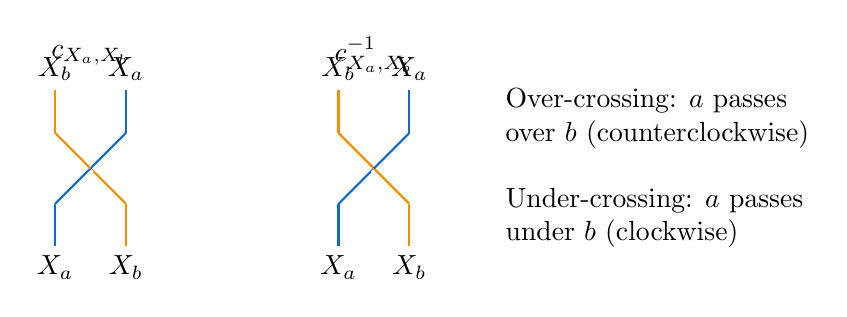
\begin{tikzpicture}[scale=0.9]
    % Over-crossing (c_{a,b})
    \begin{scope}[xshift=0cm]
        \node at (0.5, 2.7) {$c_{X_a, X_b}$};
        \draw[thick, AnyonBlue] (0, 0) -- (0, 0.6);
        \draw[thick, AnyonOrange] (1, 0) -- (1, 0.6);
        % Crossing - blue over orange
        \draw[thick, AnyonOrange] (1, 0.6) -- (0.5, 1.1);
        \draw[thick, AnyonBlue, line width=3pt, white] (0, 0.6) -- (0.5, 1.1);
        \draw[thick, AnyonBlue] (0, 0.6) -- (1, 1.6);
        \draw[thick, AnyonOrange] (0.5, 1.1) -- (0, 1.6);
        \draw[thick, AnyonBlue] (1, 1.6) -- (1, 2.2);
        \draw[thick, AnyonOrange] (0, 1.6) -- (0, 2.2);
        \node at (0, -0.3) {$X_a$};
        \node at (1, -0.3) {$X_b$};
        \node at (0, 2.5) {$X_b$};
        \node at (1, 2.5) {$X_a$};
    \end{scope}

    % Under-crossing (c_{a,b}^{-1})
    \begin{scope}[xshift=4cm]
        \node at (0.5, 2.7) {$c_{X_a, X_b}^{-1}$};
        \draw[thick, AnyonBlue] (0, 0) -- (0, 0.6);
        \draw[thick, AnyonOrange] (1, 0) -- (1, 0.6);
        % Crossing - orange over blue
        \draw[thick, AnyonBlue] (0, 0.6) -- (0.5, 1.1);
        \draw[thick, AnyonOrange, line width=3pt, white] (1, 0.6) -- (0.5, 1.1);
        \draw[thick, AnyonOrange] (1, 0.6) -- (0, 1.6);
        \draw[thick, AnyonBlue] (0.5, 1.1) -- (1, 1.6);
        \draw[thick, AnyonBlue] (1, 1.6) -- (1, 2.2);
        \draw[thick, AnyonOrange] (0, 1.6) -- (0, 2.2);
        \node at (0, -0.3) {$X_a$};
        \node at (1, -0.3) {$X_b$};
        \node at (0, 2.5) {$X_b$};
        \node at (1, 2.5) {$X_a$};
    \end{scope}

    % Explanation
    \begin{scope}[xshift=8.5cm]
        \node[align=left] at (0, 1.1) {Over-crossing: $a$ passes\\over $b$ (counterclockwise)\\\\Under-crossing: $a$ passes\\under $b$ (clockwise)};
    \end{scope}
\end{tikzpicture}
\end{center}

\begin{convention}[Crossing convention]
We use the convention that an \emph{over-crossing} (left strand passes over right) represents $c_{X_a, X_b}$, and an \emph{under-crossing} represents $c_{X_a, X_b}^{-1}$.
\end{convention}

\subsubsection{Exchange in the Fusion Tree Basis}

When the anyons are part of a longer chain with definite fusion channels, the exchange involves R-symbols:

\begin{center}
\begin{tikzpicture}[scale=0.8]
    % Before exchange
    \begin{scope}[xshift=0cm]
        \node at (1.5, -0.8) {Before};
        \draw[thick, AnyonBlue] (0, 0) -- (0, 1);
        \draw[thick, AnyonOrange] (1, 0) -- (1, 1);
        \draw[thick, AnyonTeal] (2, 0) -- (2, 1);
        \draw[thick, AnyonBlue] (0, 1) -- (0.5, 1.5);
        \draw[thick, AnyonOrange] (1, 1) -- (0.5, 1.5);
        \draw[thick, AnyonSlate] (0.5, 1.5) -- (0.5, 2);
        \draw[thick, AnyonSlate] (0.5, 2) -- (1.25, 2.5);
        \draw[thick, AnyonTeal] (2, 1) -- (1.25, 2.5);
        \draw[thick] (1.25, 2.5) -- (1.25, 3);
        \node at (0, -0.3) {$a$};
        \node at (1, -0.3) {$b$};
        \node at (2, -0.3) {$c$};
        \node at (0.8, 1.75) {$e$};
    \end{scope}

    % Arrow
    \node at (4.5, 1.5) {$\xrightarrow{R_{ab}^e}$};

    % After exchange
    \begin{scope}[xshift=7cm]
        \node at (1.5, -0.8) {After};
        \draw[thick, AnyonOrange] (0, 0) -- (0, 1);
        \draw[thick, AnyonBlue] (1, 0) -- (1, 1);
        \draw[thick, AnyonTeal] (2, 0) -- (2, 1);
        \draw[thick, AnyonOrange] (0, 1) -- (0.5, 1.5);
        \draw[thick, AnyonBlue] (1, 1) -- (0.5, 1.5);
        \draw[thick, AnyonSlate] (0.5, 1.5) -- (0.5, 2);
        \draw[thick, AnyonSlate] (0.5, 2) -- (1.25, 2.5);
        \draw[thick, AnyonTeal] (2, 1) -- (1.25, 2.5);
        \draw[thick] (1.25, 2.5) -- (1.25, 3);
        \node at (0, -0.3) {$b$};
        \node at (1, -0.3) {$a$};
        \node at (2, -0.3) {$c$};
        \node at (0.8, 1.75) {$e$};
    \end{scope}
\end{tikzpicture}
\end{center}

The fusion channel $e$ is preserved, but the amplitude acquires a factor of $R_{ab}^e$.

\subsection{Boson and Fermion Limits (\S5.1.3.4)}

The braided anyon framework correctly reproduces bosonic and fermionic statistics in appropriate limits.

\subsubsection{Bosonic Limit: $\mathsf{Vec}$}

\begin{proposition}[Bosonic exchange]\label{prop:bosonic-exchange}
For the category $\mathsf{Vec}$ (ordinary vector spaces), the braiding is trivial:
\begin{equation}
c_{V, W} : V \otimes W \xrightarrow{\sim} W \otimes V, \quad v \otimes w \mapsto w \otimes v
\end{equation}
All R-symbols are $R_{ab}^c = 1$.
\end{proposition}

\begin{corollary}
In the $\mathsf{Vec}$ limit, the exchange Hamiltonian reduces to a symmetric SWAP:
\begin{equation}
h_j^{\mathrm{ex}} = \tau \cdot \mathrm{SWAP}_j
\end{equation}
where $\mathrm{SWAP}_j$ exchanges the states at sites $j$ and $j+1$ with no phase.
\end{corollary}

\subsubsection{Fermionic Limit: $\mathsf{sVec}$}

\begin{proposition}[Fermionic exchange]\label{prop:fermionic-exchange}
For the category $\mathsf{sVec}$ (super-vector spaces) with simple objects $\mathbf{1}$ (even/bosonic) and $f$ (odd/fermionic), the braiding is:
\begin{equation}
c_{f, f} : f \otimes f \to f \otimes f, \quad c_{f,f} = -\mathrm{id}_{f \otimes f}
\end{equation}
The R-symbol for two fermions is $R_{ff}^{\mathbf{1}} = -1$.
\end{proposition}

\begin{corollary}
In the $\mathsf{sVec}$ limit, exchanging two fermions introduces a minus sign:
\begin{equation}
h_j^{\mathrm{ex}} \ket{\ldots, f, f, \ldots} = -\tau \ket{\ldots, f, f, \ldots}
\end{equation}
This is the hallmark of Fermi statistics.
\end{corollary}

\begin{remark}
The fermionic sign is automatic from the categorical structure---no additional sign factors need to be inserted by hand (compare with Jordan--Wigner transformations in spin chain approaches).
\end{remark}

\subsubsection{Anyonic Statistics: Fibonacci Example}

\begin{example}[Fibonacci R-symbols]
For Fibonacci anyons with $\tau \otimes \tau = \mathbf{1} \oplus \tau$, the R-symbols are:
\begin{equation}
R_{\tau\tau}^{\mathbf{1}} = e^{-4\pi i/5}, \quad R_{\tau\tau}^{\tau} = e^{3\pi i/5}
\end{equation}
These are neither $+1$ (bosonic) nor $-1$ (fermionic)---they are genuine anyonic phases.
\end{example}

\begin{remark}
The two different R-symbols for the two fusion channels reflect the non-abelian nature of Fibonacci anyons: the exchange phase depends on which fusion channel the pair is in.
\end{remark}

\subsubsection{Ising Anyons}

\begin{example}[Ising R-symbols]
For Ising anyons with $\sigma \otimes \sigma = \mathbf{1} \oplus \psi$:
\begin{equation}
R_{\sigma\sigma}^{\mathbf{1}} = e^{-i\pi/8}, \quad R_{\sigma\sigma}^{\psi} = e^{3i\pi/8}
\end{equation}
The $\psi$ particle (fermion) has $R_{\psi\psi}^{\mathbf{1}} = -1$.
\end{example}

\subsection{Full Classification of Two-Site Processes}

Combining hopping (\S\ref{sec:hamiltonian-v0}), interactions (\S\ref{sec:hamiltonian-v1}), and exchange, we obtain the complete set of number-conserving processes:

\begin{table}[h]
\centering
\begin{tabular}{|c|c|c|c|}
\hline
\textbf{Process} & \textbf{Morphism space} & \textbf{Requires braiding?} & \textbf{Section} \\
\hline
Vacuum identity & $\Mor(\mathbf{1} \otimes \mathbf{1}, \mathbf{1} \otimes \mathbf{1})$ & No & \S5.1.1 \\
Hop right & $\Mor(\mathbf{1} \otimes X_a, X_a \otimes \mathbf{1})$ & No & \S5.1.1 \\
Hop left & $\Mor(X_a \otimes \mathbf{1}, \mathbf{1} \otimes X_a)$ & No & \S5.1.1 \\
Two-anyon interaction & $\Mor(X_a \otimes X_b, X_c \otimes X_d)$ & No & \S5.1.2 \\
Two-anyon exchange & $c_{X_a, X_b}: X_a \otimes X_b \to X_b \otimes X_a$ & \textbf{Yes} & \S5.1.3 \\
\hline
\end{tabular}
\caption{Classification of number-conserving two-site processes.}
\end{table}

\subsection{Summary}

\begin{table}[h]
\centering
\begin{tabular}{|c|c|c|}
\hline
\textbf{Concept} & \textbf{Symbol} & \textbf{Description} \\
\hline
Braiding & $c_{X,Y}$ & Isomorphism $X \otimes Y \to Y \otimes X$ \\
R-symbol & $R_{ab}^c$ & Matrix element of braiding in fusion basis \\
Exchange term & $h_j^{\mathrm{ex}}$ & Hamiltonian term for anyon exchange \\
Free anyon Hamiltonian & $H_{\mathrm{free}}$ & Hopping + interaction + exchange \\
\hline
\end{tabular}
\end{table}

\subsection{Next Steps}

\begin{itemize}
\item \S5.2: Symmetries and conserved quantities
\item \S6: Limiting cases and verification
\end{itemize}

% \input{sections/hamiltonian_creation}

% ============================================================
% Part IV: Properties
% ============================================================
\part{Basic Properties of the Models}

% Section 6.5: Module Categories and Boundary Conditions
% module_categories.tex
% LaTeX counterpart of docs/module_categories.md
% Section §6.5

\section{Module Categories}\label{sec:module-categories}

\begin{assumption}\label{ass:module-categories}
\begin{enumerate}[label=(A\arabic*)]
    \item Fusion category $\catC$ over $\mathbb{C}$ (from \S\ref{sec:fusion-categories}).
    \item $\catC$ is rigid (has duals).
    \item Module categories are semisimple and finite.
\end{enumerate}
\end{assumption}

\subsection{Overview}

\emph{Module categories} provide the mathematical framework for classifying boundary conditions in topological phases. A (left) $\catC$-module category is a category $\mathcal{M}$ equipped with an action of the fusion category $\catC$, analogous to how a module is a set with an action of a ring.

In the context of anyonic chains, module categories classify:
\begin{itemize}
    \item Boundary conditions for open chains
    \item Edge modes and boundary excitations
    \item Domain walls between different phases
\end{itemize}

\subsection{Definition of Module Categories}

\begin{definition}[Left module category]\label{def:left-module-category}
A \emph{left $\catC$-module category} is a category $\mathcal{M}$ equipped with:
\begin{enumerate}
    \item \textbf{Action functor:} $\triangleright: \catC \times \mathcal{M} \to \mathcal{M}$, written $(X, M) \mapsto X \triangleright M$.
    \item \textbf{Module associator:} Natural isomorphism
    \begin{equation}
        m_{X,Y,M}: (X \otimes Y) \triangleright M \xrightarrow{\sim} X \triangleright (Y \triangleright M).
    \end{equation}
    \item \textbf{Unit constraint:} Natural isomorphism $\ell_M: \one \triangleright M \xrightarrow{\sim} M$.
\end{enumerate}
These satisfy coherence conditions (pentagon and triangle diagrams for modules).
\end{definition}

\begin{definition}[Right module category]\label{def:right-module-category}
A \emph{right $\catC$-module category} is defined analogously with action $\triangleleft: \mathcal{M} \times \catC \to \mathcal{M}$.
\end{definition}

\begin{definition}[Bimodule category]\label{def:bimodule-category}
A \emph{$(\catC, \mathcal{D})$-bimodule category} is a category $\mathcal{M}$ that is simultaneously a left $\catC$-module and right $\mathcal{D}$-module, with compatible associators.
\end{definition}

\begin{citationblock}
Etingof--Nikshych--Ostrik, \emph{Adv.\ Math.}\ \textbf{226} (2011) \unverified
\end{citationblock}

\subsection{Simple Module Objects}

\begin{definition}[Simple module object]\label{def:simple-module-object}
An object $M \in \mathcal{M}$ is \emph{simple} if it has no proper subobjects. The simple objects of $\mathcal{M}$ form a finite set $\Irr(\mathcal{M})$.
\end{definition}

\begin{remark}
Simple module objects correspond to \emph{boundary excitations} or \emph{edge modes}---the elementary degrees of freedom localised at the boundary.
\end{remark}

\subsection{Internal Hom}

\begin{definition}[Internal Hom]\label{def:internal-hom}
For $M, N \in \mathcal{M}$, the \emph{internal Hom} $\underline{\Hom}(M, N) \in \catC$ is defined by:
\begin{equation}
    \Hom_\mathcal{M}(X \triangleright M, N) \cong \Hom_\catC(X, \underline{\Hom}(M, N)).
\end{equation}
\end{definition}

This captures how bulk anyons ($X \in \catC$) can transform one boundary excitation into another.

\subsection{The Regular Module}

\begin{example}[Regular module]\label{ex:regular-module}
Every fusion category $\catC$ is a module over itself via the tensor product:
\begin{equation}
    X \triangleright Y := X \otimes Y.
\end{equation}
This is called the \emph{regular module} $\catC_\catC$.
\end{example}

The regular module corresponds to the ``trivial'' or ``smooth'' boundary condition.

\subsection{Module Functors}

\begin{definition}[Module functor]\label{def:module-functor}
A \emph{$\catC$-module functor} between $\catC$-module categories $\mathcal{M}$ and $\mathcal{N}$ is a functor $F: \mathcal{M} \to \mathcal{N}$ with natural isomorphisms:
\begin{equation}
    s_{X,M}: F(X \triangleright M) \xrightarrow{\sim} X \triangleright F(M)
\end{equation}
satisfying coherence conditions.
\end{definition}

Module functors describe \emph{boundary-changing operators} or \emph{defects} between different boundary conditions.

\subsection{Morita Equivalence}

\begin{definition}[Morita equivalence]\label{def:morita-equivalence}
Two fusion categories $\catC$ and $\mathcal{D}$ are \emph{Morita equivalent} if there exists an invertible $(\catC, \mathcal{D})$-bimodule category.
\end{definition}

\begin{theorem}[Boundary-bulk correspondence]\label{thm:boundary-bulk}
The bulk topological order determines, and is determined by, the set of all possible boundary conditions (module categories) up to Morita equivalence.
\end{theorem}

\begin{citationblock}
Kitaev--Kong, \emph{Commun.\ Math.\ Phys.}\ \textbf{313} (2012), 351--373 \unverified
\end{citationblock}

% boundary_conditions.tex
% LaTeX counterpart of docs/boundary_conditions.md
% Section §6.5

\section{Boundary Conditions for Anyonic Chains}\label{sec:boundary-conditions}

\begin{assumption}\label{ass:boundary-conditions}
\begin{enumerate}[label=(A\arabic*)]
    \item Bulk fusion category $\catC$ (from \S\ref{sec:fusion-categories}).
    \item 1D chain with open boundary conditions (from \S\ref{sec:lattice}).
    \item Boundary conditions classified by $\catC$-module categories.
\end{enumerate}
\end{assumption}

\subsection{Overview}

For anyonic chains with open boundary conditions, the choice of \emph{boundary conditions} at each end significantly affects the Hilbert space structure and dynamics. Following the Kitaev--Kong framework, boundary conditions are classified by \emph{module categories} over the bulk fusion category $\catC$.

Different boundary conditions lead to different edge mode structures, affecting ground state degeneracy, edge excitations, and partition functions.

\subsection{Boundary Hilbert Space}

\begin{definition}[Boundary Hilbert space]\label{def:boundary-hilbert}
For a chain with:
\begin{itemize}
    \item Bulk category $\catC$
    \item Left boundary condition $\mathcal{M}_L$ (left $\catC$-module category)
    \item Right boundary condition $\mathcal{M}_R$ (right $\catC$-module category)
\end{itemize}
The boundary-modified Hilbert space involves the \emph{relative tensor product} $\mathcal{M}_L \boxtimes_\catC \mathcal{M}_R$.
\end{definition}

\subsection{Trivial Boundary Conditions}

\begin{definition}[Trivial/smooth boundary]\label{def:trivial-boundary}
The \emph{trivial boundary condition} corresponds to the regular module $\catC_\catC$, where $\catC$ acts on itself by tensor product.
\end{definition}

Anyons can freely approach the boundary without restriction. No edge modes beyond the bulk structure.

\subsection{Gapped Boundaries via Lagrangian Algebras}

\begin{definition}[Lagrangian algebra]\label{def:lagrangian-algebra}
A \emph{Lagrangian algebra} $A \in \catC$ is a commutative algebra object satisfying:
\begin{equation}
    \dim(A)^2 = \dim(\catC),
\end{equation}
where $\dim(\catC) = \sum_i d_i^2$ is the total quantum dimension.
\end{definition}

\begin{theorem}[Classification of gapped boundaries]\label{thm:gapped-boundaries}
Gapped boundary conditions for a topological phase with bulk $\catC$ are in bijection with Lagrangian algebras in $\catC$ (for modular $\catC$).
\end{theorem}

\begin{citationblock}
Kong--Wen, \emph{JHEP} (2014) \unverified
\end{citationblock}

A Lagrangian algebra specifies which bulk anyons can ``condense'' at the boundary.

\subsection{Examples}

\begin{example}[Fibonacci anyons]\label{ex:fib-boundary}
For the Fibonacci category $\catC = \mathrm{Fib}$ with simples $\{\one, \tau\}$:
\begin{center}
\begin{tabular}{@{}lll@{}}
\toprule
Module category & Simple objects & Physical meaning \\
\midrule
$\mathrm{Fib}_\mathrm{Fib}$ (regular) & $\{\one, \tau\}$ & Smooth boundary \\
$\mathrm{Vec}$ (condensed) & $\{\one\}$ & $\tau$ condensed at boundary \\
\bottomrule
\end{tabular}
\end{center}
\end{example}

\begin{example}[Ising anyons]\label{ex:ising-boundary}
For the Ising category $\catC = \mathrm{Ising}$ with simples $\{\one, \sigma, \psi\}$:
\begin{center}
\begin{tabular}{@{}lll@{}}
\toprule
Module category & Simple objects & Physical meaning \\
\midrule
$\mathrm{Ising}_\mathrm{Ising}$ & $\{\one, \sigma, \psi\}$ & Smooth boundary \\
$\mathrm{Vec}(\mathbb{Z}_2)$ & $\{\one, \psi\}$ & $\sigma$ condensed \\
\bottomrule
\end{tabular}
\end{center}
\end{example}

\subsection{Application to Mobile Anyons}

For mobile anyons on an open chain (our setting from \S\ref{sec:hilbert-space}):

\begin{enumerate}
    \item \textbf{Standard construction} (\S\ref{sec:hilbert-space}): Uses trivial boundary conditions implicitly.

    \item \textbf{With general boundaries:} The Hilbert space becomes:
    \begin{equation}
        \catH = \bigoplus_{M_L \in \mathcal{M}_L} \bigoplus_{M_R \in \mathcal{M}_R} \catH(M_L, M_R),
    \end{equation}
    where $\catH(M_L, M_R)$ is the space of bulk configurations interpolating between boundary states.

    \item \textbf{Boundary Hamiltonians:} Additional terms can describe:
    \begin{itemize}
        \item Boundary potentials (energy cost for edge modes)
        \item Boundary-bulk coupling (anyons interacting with edge)
        \item Boundary-changing operators (transitions between boundary conditions)
    \end{itemize}
\end{enumerate}

\subsection{Connection to Golden Chain}

\begin{example}[Golden chain boundaries]\label{ex:golden-chain-bc}
The golden chain (Fibonacci anyons at unit filling) has been studied with various boundary conditions:
\begin{itemize}
    \item \textbf{Free boundaries:} Regular module, leading to CFT edge modes.
    \item \textbf{Fixed boundaries:} Specific module object pinned at edge, breaking some symmetry.
\end{itemize}
\end{example}

\begin{citationblock}
Aasen--Fendley--Mong, \emph{J.\ Phys.\ A} (2020) \unverified
\end{citationblock}


% Future sections (to be added)
% \input{sections/limiting_cases}
% \input{sections/girardeau}
% \input{sections/partition_functions}
% \input{sections/numerics}

% ============================================================
% Bibliography
% ============================================================
\bibliographystyle{alpha}
% \bibliography{../literature/references}

% Placeholder bibliography entries
\begin{thebibliography}{ENO05}

\bibitem[ENO05]{ENO2005}
P.~Etingof, D.~Nikshych, and V.~Ostrik.
\newblock On fusion categories.
\newblock {\em Annals of Mathematics}, 162(2):581--642, 2005.

\bibitem[EGNO15]{EGNO2015}
P.~Etingof, S.~Gelaki, D.~Nikshych, and V.~Ostrik.
\newblock {\em Tensor Categories}.
\newblock Mathematical Surveys and Monographs, vol.~205. American Mathematical Society, 2015.

\bibitem[Kit06]{Kitaev2006}
A.~Kitaev.
\newblock Anyons in an exactly solved model and beyond.
\newblock {\em Annals of Physics}, 321(1):2--111, 2006.

\bibitem[FTLM07]{Feiguin2007}
A.~E.~Feiguin, S.~Trebst, A.~W.~W.~Ludwig, M.~Troyer, A.~Kitaev, Z.~Wang, and M.~H.~Freedman.
\newblock Interacting anyons in topological quantum liquids: The golden chain.
\newblock {\em Physical Review Letters}, 98:160409, 2007.

\end{thebibliography}

\end{document}
